\documentclass[12pt]{scrartcl}

\usepackage[T1]{fontenc}
\usepackage[utf8]{inputenc}

\usepackage{amstext,amsmath,amssymb}
\usepackage{color}
\usepackage{dcolumn}
   \newcolumntype{d}[1]{D{.}{.}{#1}}
\usepackage{dsfont}
\usepackage{float}
\usepackage{geometry}
   \geometry{verbose,tmargin=1.4in,bmargin=1.4in,lmargin=1.4in,rmargin=1.4in}
\usepackage{graphicx}
\usepackage[hidelinks]{hyperref}
   \urlstyle{same}
\usepackage{lscape}
\usepackage[authoryear]{natbib}
   \bibliographystyle{myplainnat}

\deffootnote{1.5em}{1em}{\makebox[1.5em][l]{\thefootnotemark}}
   \setlength{\skip\footins}{1.5em}
   \setlength{\footnotesep}{1em}

\addtokomafont{disposition}{\rmfamily}

\begin{document}
\thispagestyle{empty}
\renewcommand{\thefootnote}{\fnsymbol{footnote}}
\begin{center}
{\LARGE Thinking About Need}\\\vspace{2ex}
{\Large A Vignette Experiment on\\[1ex] Need-Based Distributive Justice}\\ \vspace{6ex}
{\large Alexander Max Bauer,$^a$\footnotemark[1] Adele Diederich,$^b$\\Stefan Traub,$^{c}$ Arne R. Weiss$^{d,\,e}$}\\ \vspace{3ex}
\textsl{\small $^{a}$Dept. of Philosophy, University of Oldenburg, Oldenburg, Germany}\\\vspace{1ex}
\textsl{\small $^{b}$Dept. of Psychology, University of Oldenburg, Oldenburg, Germany}\\\vspace{1ex}
\textsl{\small $^{c}$Dept. of Economics, Helmut-Schmidt-University, Hamburg, Germany}\\\vspace{1ex}
\textsl{\small $^{d}$Dept. of Economics, University of Alicante, Alicante, Spain}\\\vspace{1ex}
\textsl{\small $^{e}$Wyss Academy for Nature, University of Bern, Bern, Switzerland}\\\vspace{4ex}

\end{center}

\vspace{\fill}

\noindent\textbf{Abstract:} We examine the role of need satisfaction in non-comparative justice ratings of endowments with goods.
As normative approaches, we discuss utilitarianism, prioritarianism, and three versions of sufficientarianism.
Using a vignette experiment with $109$ participants, we elicit the participants' justice ratings of endowments with living space and estimate their justice evaluation functions.
We show that a need context increases the prevalence of prioritarianistic and sufficientarianistic justice ratings.
Moreover, a need threshold also changes the utilitarians' justice evaluation functions significantly.
\\[2ex]
\noindent\textbf{Keywords:} Basic Needs, Justice Principles, Prioritarianism, Sufficientarianism, Utilitarianism, Vignette Experiment\\[2ex]
\textbf{JEL Classification:} I30, D63, D31

\footnotetext[1]{Corresponding author.
Department of Philosophy, University of Oldenburg, Ammerl{\"a}nder Heerstra{\ss}e 114--118, 26129 Oldenburg, Germany, \href{mailto:alexander.max.bauer@uni-oldenburg.de}{alexander.max.bauer@uni-oldenburg.de}.
Telephone: +49 (0)441 798 2034.}
\renewcommand{\thefootnote}{\arabic{footnote}}\setcounter{footnote}{0}
\newpage


%%%%%%%%%%%%%%%%
% INTRODUCTION %
%%%%%%%%%%%%%%%%
\section{Introduction}\label{sec:introduction}
How do laypeople evaluate the justice of personal endowments with goods that satisfy basic needs?
\cite{miller_principles_1999} emphasizes that needs are not to be confused with wants; needs rely on a socially shared notion.
Need, then, refers to whether someone has \textit{enough} \citep{frankfurt_inequality_2015} to live a \textit{decent life} \citep{miller_principles_1999}.
The question of whether someone has enough points to the \textit{non-comparative} \citep{feinberg_noncomparative_1974} thrust of need as a criterion of justice: It is human suffering due to unfulfilled needs that causes injustice, not how one is treated relative to others.
This raises the question of how justice is related to the satisfaction of need, to which the literature offers no precise answer.

In this paper, we first discuss the \textit{non-comparative} dimension of need-based distributive justice using three normative approaches: utilitarianism \citep[e.\,g.,][]{bentham_introduction_2009,mill_utilitarianism_1998}, prioritarianism \citep[e.\,g.,][]{parfit_equality_1997}, and sufficientarianism \citep[e.\,g.,][]{frankfurt_equality_1987,crisp_egalitarianism_2003,schramme_is_2006}.
We then present an empirical investigation of justice ratings of laypeople using a vignette experiment.
In the vignette experiment, we asked participants to rate different endowments with living space in terms of justice.
An explicit need threshold was communicated in a Need treatment and was absent in a control treatment.
Additionally, to test the robustness of the results, there were two different rating tasks.
In the global rating task, 11 scenarios of endowment with living space had to be rated individually.
In the relative rating task, pairs of scenarios had to be evaluated in comparison to each other.

We examine whether the communication of a threshold in the Need treatment leads to a change in the proportions of individual justice ratings that are consistent with utilitarianism, prioritarianism, and sufficientarianism.
Methodologically, our approach to measuring the \textit{perceived} justice of endowments with living space using a vignette experiment is inspired by empirical justice research \citep[for an overview see, e.\,g.,][]{sabbagh_handbook_2016} and, in particular, the work of sociologist Guillermina Jasso and her co-authors on the justice of earnings \citep[see, e.\,g.,][]{jasso_distributive_1977,jasso_justice_1978,jasso_methods_1990,jasso_how_1999}.
Like Jasso, we assume that a Justice Evaluation Function (JEF) exists that maps the set of a person's endowments with living space onto a set of justice ratings.
However, as will be explained in detail below, our approach differs from Jasso's with respect to the justice scale and its interpretation (we use a psychometrical instead of a psychophysical function), the specification of an explicit reference point in the Need treatment, and the examination of individual heterogeneity with respect to the participants' normative considerations of justice.

Vignette experiments have become the de facto methodological standard for empirical justice research because they promise both experimental control of predictor variables (in our case: need satisfaction) and external validity for situations that, for ethical or practical reasons, cannot be studied in real-life situations (see \citealp{bardsley_experimental_2009}; for overviews see \citealp{traub_friedman_2005,gaertner_empirical_2012}).
This clearly applies to research on human needs.
While this paper is not the first to empirically study the role of needs for justice evaluations,\footnote{The first was \cite{yaari_dividing_1984}. Recent examples include \cite{kittel_impact_2020,wyszynski_give_2023}. For an overview see \cite{traub_need-based_2020}.} we are not aware of any empirical work, nor a conceptual framework for that matter, that can shed light on the precise relationship between need satisfaction and justice ratings.

Our main results are as follows: The analysis of the individual justice ratings shows that a large proportion of the participants can be assigned to one of the three main justice types: sufficientarianism, prioritarianism, or utilitarianism.
The need threshold treatment significantly shifts the distribution of justice ratings in favor of sufficientarianism and prioritarianism.
The analysis of the absolute average justice ratings shows that an exogenous need threshold for endowment with living space leads to a \textit{sigmoid} JEF.
Below the need threshold, the JEF is convex and justice ratings are lower than without a need threshold.
If the endowment with living space is at least as high as the need threshold, the JEF is concave and the ratings close to the need threshold are significantly above the ratings without a need threshold.
This rating pattern is confirmed by the analysis of the relative justice ratings.

Our vignette experiment therefore contributes to answering the question of how laypeople think about need-based justice.
In our setting, where the focus lies on the non-comparative dimension of justice ratings, need significantly changes both individual and mean justice ratings.
However, this also means that individual and aggregated evaluations of justice are dependent on the framing of the situation being assessed.

The remainder of the paper is organized as follows.
In the next section, we provide a review of the relevant literature.
Our methodological approach is explained in Section \ref{sec:methodology}, and the design of our vignette experiment is presented in Section \ref{sec:experiment}.
The results of the experiment are shown in Section \ref{sec:results}.
The paper ends with a summary and discussion of the results in Section \ref{sec:conclusion}.


%%%%%%%%%%%%%%
% LITERATURE %
%%%%%%%%%%%%%%
\section{Literature Review}\label{sec:background}


%%%%%%%%
% NEED %
%%%%%%%%
\subsection{The Concept of Need}\label{sec:need}
Needs influence our thinking in many areas.
Take, for example, social policy.
Here, one might think of minimum wage or---especially---of \textit{means-tested benefits}, which are an essential element of the liberal (i.\,e., mostly Anglo-Saxon) ``World of Welfare Capitalism'' \citep{esping-andersen_three_1990}.
Means-tested benefits stand in the tradition of the ``poor laws'' that differentiated between deserving and undeserving poor.
This distinction---in itself already a separation between the needy and the not-needy---lives on, for example, in the United States welfare system.
Here, only those who fulfill certain criteria, such as the presence of a disability or a pregnancy, are eligible for benefits from the governmental health program ``Medicaid''---but only if they also have an insufficient income under a poverty threshold which was initially defined by congress as a triple the amount needed for basic nutrition in the year 1963 and is adjusted for inflation annually.
This poverty threshold can be seen as a collectively determined concept of basic need, which serves as a guideline for social policy.

This is also the case for the ``applicable amount'' defined by the government of the United Kingdom, which was (and still is, in the case of the ``Universal Credit'' program) the reference point for the government's old welfare programs.
In conservative, contribution-based welfare states like Germany, need also plays a crucial role in the provision of welfare.
The means-tested and workfare-based unemployment allowance ``Arbeitslosengeld II'' (replaced by the ``B{\"u}rgergeld'' as of 2023) defines a household consisting of family members or mutually dependent residents explicitly as a ``Bedarfs\-gemeinschaft''---a companionship with a shared need.
This need is defined following a statistically assembled consumer basket and adjusted annually following the development of prices and wages.
In like manner, the ``BAf{\"o}G'' (``Federal Law on Support in Education'') defines how much students need for their livelihood.
Corresponding to the central role of the family in the conservative welfare state and its principle of subsidiarity, the student's parents are primarily responsible for providing the student's livelihood.
Only if their income is insufficient will the government fill the resulting gap by granting benefits that consist of equal shares of a grant and an interest-free loan.

The concept of need can also be found when it comes to the assessment of poverty.
Besides the measures of relative and absolute poverty, another poverty indicator that strongly corresponds with the idea of need is the concept of ``material deprivation''.
Here, sets of items are used to evaluate whether an individual can be considered ``materially deprived''.
These sets vary, but in many cases include basic needs such as the ``ability to adequately heat the dwelling'', the ``ability to have a healthy diet'', the ``ability to clothe properly'', or ``access to health care'' \citep[p.~37]{boarini_measures_2006}.
Needs, therefore, do not only play a role in the formulation of policies but also when it comes to assessing whether there is a necessity for political intervention or when it comes to evaluating if the actions taken were successful.

Besides these practical and evaluative perspectives, need has---as \cite{bauer_need_2022} have pointed out---also been of importance in political theory \citep{dean_translation_2013,doyal_theory_1984,nussbaum_human_1992,weale_political_1984}.
It has been suggested by many as a fundamental cornerstone for human rights \citep[e.\,g.,][]{brock_needs_2005,gasper_needs_2005,renzo_human_2015} and has also gained traction in positive justice research \citep[for a summary of some recent work, see, e.\,g.,][]{miller_needs-based_2020}.
While early empirical research on distributive justice attitudes in the 1960s and 1970s focused on \textit{equity theory}, this focus changed during the 1970s and 1980s with, for example, \cite{deutsch_equity_1975} arguing that such a singular approach confounds distinct allocation principles.\footnote{Note that Deutsch limits the relevance of needs to a much narrower sphere than we do. Recent research has shown that the principle of need---contrary to Deutsch's assumption---also plays a role beyond such close personal relationships.}
Instead, he suggested studying equity, equality, and need as different principles.
In a similar manner, \cite{schwinger_just_1980} suggested contribution, equality, and need.
\cite{wagstaff_equity_1994} proposed equity, equality, and need, and \cite{konow_fair_2001} equity, efficiency, and need.
As \cite{konow_is_2009} notes, empirical investigations increasingly find preferences for unequal distributions, giving room for principles other than equality.
Concerning need, it is notable that people were found to prefer distributions that comply with securing floor levels \citep[e.\,g.,][]{ahlert_thresholds_2012,frohlich_choosing_1992,frohlich_choices_1987}.

But, after all, what \textit{is} a need?
As \cite{bauer_need_2022} have summarized, a need can be defined as a necessity of a good which is required by a person to avoid being harmed.
Such needs can be biological (e.\,g., the need for hydration or nutrition) or social (as in the famous example of a worker needing a linen shirt put forth by Adam \citealt{smith_wealth_1979}).
Needs are not to be confused with wants; needs rely on a socially shared notion \citep{miller_principles_1999}.
An individual may have such a strong preference for eating bluefin tuna that she feels pain whenever it is not part of her menu.
For this want to become a need, however, others must \textit{acknowledge} that eating bluefin tuna is necessary in order for her not to be harmed (which in this case seems fairly unlikely).
As an inter-subjectively acknowledged threshold, needs provide a fundamentally different basis of social justice than other criteria, such as equality, equity, or the Rawlsian maximin principle \citep[for philosophical overviews on need-based justice, see][]{miller_needs-based_2020,siebel_need_2020}.

How the need criterion can be distinguished from the latter is its defining question: Do people have enough \citep{frankfurt_inequality_2015} to lead a minimally decent life \citep{miller_principles_1999}?
This question shows the \textit{non-comparative} \citep{feinberg_noncomparative_1974} thrust of need-based justice: It is, first of all, human suffering due to unfulfilled needs that causes injustice, not how one is treated relative to others.
This raises the question of how justice is related to need satisfaction, to which the literature offers no precise answer.

The main reason for this gap might lie in the focus of many accounts of social justice on the \textit{comparative} dimension of justice, that is, how one person's dues are related to how much other members of society receive.
This is clearly an important endeavor, and a focus on need does not make it obsolete.\footnote{The comparative dimension is always present when members of society differ in important aspects and need considerations stop carrying much weight when everyone's needs are fulfilled.}
However, there seems to have been little progress in reaching common principles of comparative justice accepted by involved parties with their differing interests and their selfishly biased perceptions.

Seeing justice through the lens of need satisfaction, however partial that perspective may be, might have a vital upshot: Since need thresholds are based on a shared understanding within society, need-based justice may have the chance to reach a consensus, even among involved parties, that harm should be avoided, regardless of a suffering person's deserts, status, or responsibility.
The relative silence in the literature on the relationship between need satisfaction and justice is, therefore, an important gap: If all we can say is that unnecessary suffering is unjust, how can we, as theorists or policy-makers, differentiate between situations with \textit{different levels of suffering} or decide between situations that involve trade-offs between members of society?

In this paper, we focus solely on the non-comparative dimension of justice, hitherto largely neglected in both the empirical and the normative literature.\footnote{A comparative measure of need-based justice, which is based on the inequality of unsatisfied need, was developed by \citet{miller_principles_1999}. For a critical discussion, see \citet{siebel_need_2020}. For a more recent comparative measure of need-based justice, see \citet{springhorn_measurement_2022}.}
Against this background, we will present empirical data based on evaluations of participants acting as \textit{impartial spectators} in a vignette experiment.
As many have argued (see, e.\,g., \citealp{konow_which_2003}, and \citealp{miller_distributive_2017}), the impartial views of real people are a crucial foundation for political and normative theory.
Asking laypeople helps the theorist to go beyond and possibly question her own pre-theoretical intuitions.
Not least, for a theory of justice to be capable of reaching a consensus, it has to be accepted by non-experts \citep[also see][]{de_vries_empirical_2009,bauer_empirical_2020}.


%%%%%%%%%%%%%%
% PRINCIPLES %
%%%%%%%%%%%%%%
\subsection{Principles of Justice and the Justice Evaluation Function}\label{sec:principles}
How is need related to different principles of justice?
It seems a clear point of departure to characterize a situation of unfulfilled needs as less just than a situation in which needs are fulfilled \citep{kipnis_economic_1985}.
This follows straightforwardly from several accounts of justice which acknowledge a non-comparative dimension, such as utilitarianism, prioritarianism, or sufficientarianism (variations of these theories will be coming up again later when we evaluate the individual data of our participants, see Section \ref{sec:individual}).\footnote{It may even be deduced from the writings of Plato and Cicero \citep[see][]{siebel_each_2017}.}
While utilitarianism focuses on the overall outcome \citep[e.\,g.,][]{bentham_introduction_2009,mill_utilitarianism_1998}, prioritarianism puts extra weight on the well-being of those who are particularly ill off \citep[e.\,g.,][]{parfit_equality_1997}, and sufficientarianism strives for everyone to have at least enough \citep[e.\,g.,][]{frankfurt_equality_1987,crisp_egalitarianism_2003,schramme_is_2006}.
This is not to say that these---primarily non-comparative---principles leave no room for comparative principles, such as egalitarianism, to enter.

Moreover, one may differentiate between \textit{qualitative} and \textit{quantitative} accounts of need-based justice \citep[see][]{siebel_need_2020}.
A purely qualitative principle is ``binary'' in that---after having identified a need---it simply differentiates between just and unjust endowments without making a statement about how just or unjust the endowment with the respective good or service is.
A quantitative principle additionally makes it possible to measure (and compare) the degree of need-satisfaction, but it involves measurement and scaling issues \citep[see][]{diederich_identifying_2020}.

Suppose that, for each individual, a quantitative measurement of justice that is based on the satisfaction of basic needs exists---a (cardinal, real-valued) Justice Evaluation Function (JEF).
Then, further questions arise about its properties, particularly regarding its shape around the need threshold (i.\,e., the point of complete need satisfaction).
First, precisely how does justice rise below the need threshold (``undersupply'')? Second, what does the shape of the JEF look like beyond the need threshold (``oversupply'')?

From the utilitarian point of view, it can be assumed that more living space leads to greater well-being (as long as there is no trade-off with other goods, as we assume).
Accordingly, an endowment with living space is just if it maximizes living space.
In other words, since a greater endowment increases well-being, the just thing is to provide it.
Hence, the JEF also rises in situations of ``oversupply'', which implies that it does not reach its maximum value at the need threshold.
Thus, the utilitarian JEF is an \textit{increasing} function of living space both \textit{below and above} the need threshold.

Prioritarianism gives more weight to the well-being of those who are badly off.
According to \citet{arneson_egalitarianism_2002}, injustice is directly linked to a person's suffering (and not to the level of inequality), which gets progressively worse the lower the endowment is.
Strictly speaking, providing less than what is needed leads to suffering and is then undifferentiatedly unjust.
Thus, the ``strictly'' prioritarian JEF is \textit{zero below} the need threshold and an \textit{increasing} function of living space \textit{above} the need threshold.\footnote{This particular definition of strict prioritarianism is related to the decision scenario of our experiment and is used to distinguish between the principles of justice in terms of the shape of the Justice Evaluation Function.}

Sufficientarianism, by contrast, gives a completely different answer by putting a particular moral significance on a person reaching the sufficiency line.
For a corresponding sufficiency line, a person's need is the most plausible candidate.
Therefore, the JEF reaches its maximum value at the need threshold.\footnote{However, this does not preclude other considerations, such as utilitarianism, from entering. Roger Crisp's \citeyearpar{crisp_egalitarianism_2003} account of sufficientarianism can be understood along these lines and suggests utility maximization beyond the sufficiency line \citep[see][]{arneson_egalitarianism_2002}.}
In the following, we distinguish qualitative, quantitative, and strict sufficientarianism:
A ``qualitative'' sufficientarian regards all endowments below the need threshold as undifferentiatedly unjust, but endowments that are at least sufficient as perfectly just.
Hence the JEF is \textit{binary} with a \textit{jump from zero to one} at the need threshold.
A ``quantitative'' sufficientarian, on the other hand, rates higher endowments below the sufficiency line as more just, i.\,e., the JEF is \textit{increasing} in living space below and \textit{flat at and above} the need threshold.
Moreover, one could argue that for sufficientarianism, enough is enough.
Consequently, the ``strictly'' sufficientarian JEF would be hump-shaped, i.\,e., \textit{increasing below} and \textit{decreasing above} the need threshold.

Any purely comparative notion of justice, such as egalitarianism, implies a flat justice evaluation at its maximum value since households are always treated equally.
The implausibility of this implication is precisely what drives the leveling-down objection \citep{nozick_anarchy_1974,raz_morality_1986,temkin_inequality_1993}  against egalitarianism and shows that we also need an explicit treatment of the non-comparative dimension of justice.\footnote{In fact, in the debate between prioritarians and egalitarians about the leveling-down objection, the separability between the non-comparative dimension (the personal benefits of the people) and the comparative dimension (inequality among the people) of overall welfare plays an important role \citep[for a careful analysis see, e.\,g.,][]{jensen_what_2003}. In our study, however, we deliberately omit all contexts other than the personal benefits of the representative household and its need to be provided with living space.}

To summarize this discussion, different (primarily non-comparative) theories of justice imply different shapes of the JEF.
In order to test whether the normative considerations underlying these theories are echoed in individual justice ratings of laypeople, we designed a vignette experiment that is explained in detail in Section \ref{sec:experiment}.
Our experiment tests whether the introduction an explicit need threshold (in terms of being able to live a decent life) changes the participants' non-comparative justice attitudes with respect to hypothetical endowments with units of living space.

Before we present the methodology in detail in the next section, we briefly distinguish the concept of need-based justice from the concept of poverty.
Poverty measurement is known to have two central steps: identification and aggregation \citep[for excellent surveys of the literature on poverty measurement, see][]{seidl_poverty_1988,zheng_aggregate_1997}.
Identification determines who is poor by defining the poverty line.
Depending on the concept, this threshold may be absolute (e.\,g., the income needed to maintain physical fitness), relative (e.\,g., a percentage of the median income), or subjective (e.\,g., in the sense of a feeling of relative deprivation).
In contrast to these approaches, the concept of need-based justice is based on an intersubjective understanding of what is needed in a society in order to lead a decent life.
Need-based justice, thus, is most closely related to the concept of absolute deprivation proposed by \citet{sen_poverty_1981}.
Ultimately, however, Sen's concept is also relative, because the focus is on a person's relative deprivation in terms of commodities, income, and resources, which results from her absolute deprivation in terms of her capabilities.

The second step, aggregation, then measures the extent and intensity of poverty using ad hoc or axiomatic indices.
Sen's \citeyearpar{sen_poverty_1976} focus axiom, e.\,g., demands that the measure of poverty must not depend on the income of the rich.
There are different variants of the transfer axiom that determine how progressive transfers\footnote{The transfer principle is attributed to \citet{pigou_wealth_1912} and \citet{dalton_measurement_1920}.} between the poor (and between the poor and the rich) affect poverty.
In contrast to this, we do not aggregate over the set of the poor, but rather measure the justice of endowing a representative household with different units of living space individually, both falling below and meeting or exceeding the need threshold.\footnote{Note that, in her later work, Jasso derived various aggregate measures of justice from her JEF and axiomatized them \citep[see, e.\,g.,][]{jasso_how_1999}.}
However, the gap between the perfectly just and the actual endowment of an undersupplied household can be interpreted as a kind of ``justice gap'', analogous to the ``relative poverty gap'' in poverty measurement, which reflects its absolute deprivation.\footnote{\citet{duclos_absolute_2002} show a very interesting way of separating absolute from relative deprivation in poverty indices.}
As said before, we do not weigh these justice ratings against each other, nor do the three \textit{non-comparative} principles of justice, whose empirical relevance we want to investigate in this study.


%%%%%%%%%%%%%%%%%%%%%%%%%%
% METHODOLOGICAL REMARKS %
%%%%%%%%%%%%%%%%%%%%%%%%%%
\section{Methodology}\label{sec:methodology}
Our empirical approach to measuring the perceived justice of households' endowments with living space given their need is based on \textit{psychophysical scaling}.
The term ``refers to the process of quantifying mental events, especially sensations and perceptions, after which it is possible to determine how these quantitative measures of mental life are related to quantitative measures of the physical stimuli'' \citep[p.~91]{marks_psychophysical_2002}.
The abundant literature on psychophysical scaling has shown that the findings of psychophysics on sensation and perception (such as the Weber-Fechner law and Steven's power law) can be transferred to \textit{social phenomena} such as the strength of support for a political party \cite[see, e.\,g.,][]{stevens_psychophysics_1986}.
\citet[pp.~617--618]{lodge_psychophysical_1975} give numerous early examples of applications for social research.
More recently, \citet{osmundsen_psychophysiology_2022} evaluate psychophysiological correlates of political ideology, such as the electrodermal activity, in a meta-study.
A basic prerequisite for our study, therefore, is that such a psychophysical transformation process exists that maps the ``objective reward criterion''---living space---onto the ``subjective world''---the justice rating \citep[p.~412]{jasso_methods_1997}.\footnote{Note, however, just like Jasso, we do not measure psychophysical correlates of the perceived justice of endowments with living space.}

In psychophysics two prominent classes of functions are discussed: A psychometrical function relates the detection or discrimination of physical stimuli to relative frequencies (probabilities); and a psychophysical function maps physical entities onto a psychological scale such as sensation, perception, or any other mental events \citep[p.~91]{marks_psychophysical_2002}.
Using a psychophysical approach, Jasso and colleagues intensively studied the justice of earnings \citep[e.\,g.,][]{jasso_distributive_1977,jasso_justice_1978,jasso_methods_1990,jasso_methods_1997,jasso_how_1999}.
The concrete form of the psychophysical function is determined by the stimulus and the type of psychophysical experiment.
For example, \citet[p.~138]{jasso_how_1999} constructed a Justice Evaluation Function (JEF) which describes the justice of earnings by the natural logarithm of the ratio between actual reward $A$ over just reward $C$ multiplied with a constant $\theta$, $J_\text{Jasso}=\theta\ln(A/C)$.\footnote{The logarithmic form was initially a purely empirical result based on vignette studies. In general, the \textit{signature constant} $\theta$ represents the framing and the expressed justice. It is positive for rewards and negative for punishments or burdens. Its absolute value varies with the scale and the individual justice attitude.}
This function corresponds to the Weber-Fechner law according to which an exponential increase in the stimulus above the stimulus threshold only produces a linear increase in the intensity of sensation \cite[see][p.~409, and the literature stated therein]{jasso_methods_1997}.

In our experiment, which is presented in more detail in the following section, the participants solve a ``Thurstonian'' \textit{discrimination task} \citep[pp.~101--104]{marks_psychophysical_2002}.
The experiment consists of a vignette in which the issue of building $x\in\mathbb{R}:\{x\ge0\}$ units of living space for a representative household is introduced.
In the status quo, the household has nothing, $x_{sq}=0$.
Throughout the task, we keep $x_{sq}$ constant and vary $x$.
In psychophysics, the ``method of constant stimuli'' is used to check whether participants are able to discriminate between $x$ and $x_{sq}$.
The participants' cumulative responses to the differing levels of contrast, $c=x-x_{sq}=x$, can then be used to estimate a psychometrical function, such as the Weibull function \citep{wichmann_psychometric_2001,mortensen_additive_2002}, which describes the \textit{probability} that participants evaluate the stimulus $x$ as exceeding the comparison stimulus $x_{sq}$ \citep[p.~2503]{treutwein_adaptive_1995}.\footnote{The basic idea that the ability to discriminate between two stimuli of different sizes is probabilistic and depends on the size of the stimuli goes back to \citet{fechner_elemente_1860}. It can be found analogously in the discrete choice literature, in which the fact that individuals do not always behave consistently when choosing between two alternatives is taken into consideration by adding an error term to the difference in the latent utility of the alternatives, which is why this model is also called the Fechner model \citep[see, e.\,g.,][]{blavatskyy_fechner_2018}.}
In other words, we investigate whether the participants find the potential endowment ($x$) more just than no endowment ($x_{sq}=0$) at all and whether the explicit specification of a need threshold influences this evaluation.

\begin{figure}[h!t!]
   \centering
   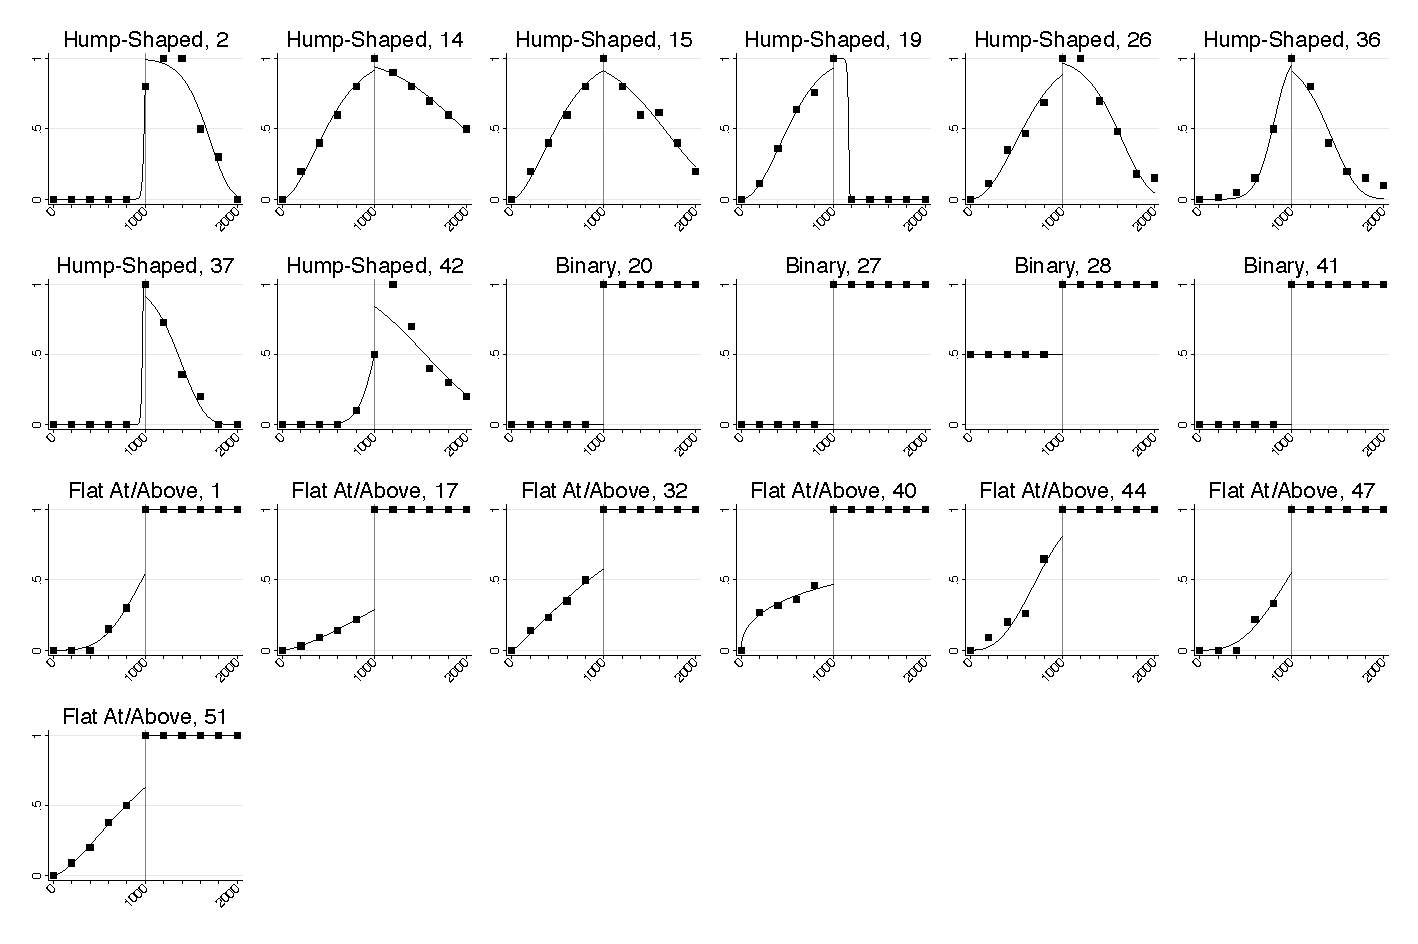
\includegraphics[width=0.5\linewidth]{figures/figure_1.pdf}
   \begin{minipage}{\linewidth}
   \footnotesize
   \textit{The figure shows the theoretical shape of the Weibull function $J(c)$ for stimuli between $0$ and $2000$ units of living space for $3$ different shape parameters $k$. The dispersion parameter $\lambda$ is adjusted in each case so that $J(2000)=0.95$. For $k=2$, the inflection point from convex to concave occurs at $c=817$.}
   \end{minipage}
   \caption{Shapes of the Weibull function}
   \label{fig:figure_1}
\end{figure}

The psychometrical function of our choice is the Weibull distribution $J(c)=1-\exp(-\lambda c^k)$, $\{c\in\mathbb{R}:c\ge0\}$, which is often used in psychometric research \citep{wichmann_psychometric_2001,mortensen_additive_2002}.
Figure \ref{fig:figure_1} shows the theoretical shape of the function for different parameterizations.
Since $J(c)$ is a distribution function, the justice scale is defined on the closed unit interval $J\in[0,1]$, where an allocation is ``perfectly unjust'' if $J=0$ and ``perfectly just'' if $J=1$.
The exponent $k$ is called the ``shape parameter''.
If $k<1$, the mean justice rating of the stimulus increases at a \textit{decreasing} rate.
If $k=1$, the Weibull reduces to an exponential distribution and the justice rating increases at a \textit{constant} rate.
In both cases $k\le 1$, $J(c)$ is concave.
If $k>1$, the justice rating increases at an \textit{increasing} rate up to an inflection point.
Hence, it is convex below and concave above the inflection point, i.\,e., it is \textit{sigmoid}.
$\lambda$ is called the ``scale parameter'' and yields the dispersion of justice ratings.\footnote{In contrast to this, $J_\text{Jasso}$ is concave and nondecreasing in the reward ratio. The measure takes a value of $0$, representing perfect justice, if actual reward and just reward are identical; it takes negative values in case of unjust allocations; and positive values in case of reward ratios exceeding $1$.}

In the Need treatment of our vignette experiment, we additionally inform about a need threshold, $x_\text{need}$, that could serve as a subjective reference point for evaluating the contrast, i.\,e., the potential endowment with living space.
For example, as discussed in Subsection \ref{sec:principles}, a qualitative sufficientarian with reference point $r=x_\text{need}$ would rate any endowment $x\in[0,x_\text{need})$ as perfectly unjust and any endowment $x\in[x_\text{need},\infty)$ as perfectly just.
These justice ratings can then be interpreted psychometrically in terms of a \textit{probability}, i.\,e., $J=1$ means that the qualitative sufficientarian is $100\%$ sure that building $x\ge x_\text{need}$ units is just, or in terms of the \textit{strength of a social preference}, the sufficientarian would agree to $100\%$ that $x$ units of living space should be built for the representative household.
The experimental design also allows us to estimate JEFs for groups of participants whose ratings conform with one of the normative principles or for the whole sample in order to study justice perceptions at the aggregate ``societal'' level.


%%%%%%%%%%%%%%
% EXPERIMENT %
%%%%%%%%%%%%%%
\section{The Experiment}\label{sec:experiment}
First, in Subsection \ref{sec:treatments}, we explain the experimental design.
In Subsection \ref{sec:expectations}, we present expectations for the results of the experiment.
Subsection \ref{sec:procedure} provides information about the sample and how the experiment was implemented.


%%%%%%%%%%%%%%
% TREATMENTS %
%%%%%%%%%%%%%%
\subsection{Treatments}\label{sec:treatments}
In the main treatment (Need) of our vignette study, we asked participants to imagine that only the state could meet people's need for housing.
Needs were presented as a fictitious amount of living space ($1000$ units per household) that residents of the region consider necessary for a \textit{decent life}.
Participants were told that space of this size means ``to live in close quarters'', but it is ``just enough to lead a decent life''.
They were also informed that households do not differ in any other meaningful way, ruling out considerations of deserts, accountability, and so forth, and that they prefer more to less living space.

Moreover, the means at the state's disposal are sufficient to build up to $2000$ units per household.
The regional parliament decides how many units will actually be built.
By informing participants that this decision has no other noteworthy consequences, we wanted to avoid that they considered possible opportunity costs of building living spaces and make clear that utilitarian concerns would call for building the maximum amount possible.
In the control treatment (NoNeed), the vignette was the same but without the parts that relate to needs (see the exact wording of the vignette in Appendix \ref{sec:app_vignette}).

Participants rated $11$ scenarios that differed in the endowment with living space provided by the state for each household.
The potential endowment ranged from $x=0$ to $x=2000$ units in equal steps of $200$ units.

There were two different rating tasks: In the \textit{global} rating task, participants directly rated each scenario separately on a scale from $0$ to $100\%$, where $100\%$ was presented as ``perfectly just'' and lower numbers meant correspondingly lower degrees of justice.
In the \textit{relative} rating task, participants evaluated the perceived difference in justice between two scenarios that were adjacent in terms of endowment (e.\,g., $0$ versus $200$ units) on an $11$-point Likert scale.
On this scale, $1$ represents indifference (``equally just/unjust''), while $11$ means that one scenario was deemed ``much more just''.
In order to control for ordering and anchoring effects, the presentation of endowments and the initial slider position were randomized.
Participants were told that they would have to move the slider at least once in each scenario.
If a subject left the slider at the starting position, a missing value was recorded.

Each subject was assigned to either the Need or the NoNeed task (between-participants treatment).
All participants were presented with both the global and the relative rating task in randomized order (within-participants treatment).\footnote{The order of the tasks was irrelevant for the average justice ratings in the global rating task. In the relative ratings task, however, the average justice ratings of the differences between two endowments were significantly lower when the global ratings task was conducted first ($p=0.018$).}

Recall that our \textit{global} rating scale for how ``just'' the endowment is, ranges from 0 to 100 percent for the $11$ equally distant endowments.
It is well known from measurement theory that bunching may occur at extreme values \citep[e.\,g.,][]{mickes_strong_2011} if respondents want to maximize the information content of their ratings in case there is more uncertainty about how to rate a medium stimulus compared to an extreme stimulus (a theoretical treatment of the issue is given by \citealt[p.~1652ff.]{seidl_how_1994}).
For the global rating task, this could mean that the lowest or highest endowment category is mapped onto a small range of extreme justice ratings, i.\,e., a small range of very low or high percentages on the justice scale, respectively, while the medium endowment category (close to the need threshold) is mapped to a relatively large range of medium percentages.
Hence, bunching would then ``technically'' cause a \textit{sigmoid} JEF, where the shape of the JEF is related to uncertainty rather than non-comparative justice principles.

In order to address the bunching concern, we conduct the \textit{relative} rating task, which provides participants with a new rating scale for every pair-wise comparison, as a robustness check.
Since participants first have to decide which of the two levels of endowment they perceive as \textit{more} just and then have to decide upon the \textit{magnitude} of the difference on an $11$-point Likert scale, the rating scale effectively runs from $-10$ to $+10$, with negative values indicating that the smaller endowment is rated as more just.


%%%%%%%%%%%%%%%%
% EXPECTATIONS %
%%%%%%%%%%%%%%%%
\subsection{Expectations}\label{sec:expectations}
What does the JEF of the participants in the experiment look like?
Does explicitly defining a minimum amount of living space, under which living a decent life in the community is not possible, cause different justice ratings in the Need treatment as compared to the NoNeed treatment?
In the following, we derive some expectations as to the treatment effect of the need threshold on the justice ratings and the shape of the JEF in line with our discussion of justice principles in Subsection \ref{sec:principles} and the methodological considerations in Section \ref{sec:methodology}.

Our expectation for the NoNeed treatment is as follows.
Since there is no explicit evidence in terms of a threshold for prioritizing the needs of certain households or sufficiency considerations, utilitarian considerations are likely to prevail.
Thus, we expect the JEF of most participants to increase monotonically from $0$ to $2000$ units of living space, because more living space means greater well-being and, thus, more justice.
While $J(0)=0$ seems obvious, $J(2000)$ could well be less than $1$ if it were conceivable that more resources than the $2000$ units would be made available for building living space.

In the Need treatment, we expect the need threshold of $1000$ units to become a reference point that changes the evaluation of the potential endowment with units of living space below, at, and above the need threshold.
Our expectation is that the proportion of utilitarian justice evaluations will decrease and the proportion of prioritarian (zero below the need threshold) and sufficientarian (hump-shaped, binary, or flat at and above the need threshold) justice evaluations will increase.

There may be exceptions for participants exhibiting a purely comparative justice attitude, such as egalitarian distributive preferences.
They would perhaps disagree that the rating task is related to justice at all and, therefore, refuse to execute the task.
Alternatively, egalitarian participants might state flat justice ratings at the maximum value of $100\%$ because the vignette implies that all households in the community receive the same endowments with living space.
Moreover, we should see no treatment effect among egalitarians with respect to need.

For the relative rating task, our hypotheses imply that relative justice ratings are expected to be non-negative since the justice evaluation is nondecreasing in living space except for strict sufficientarians.
Furthermore, we expect the relative justice ratings to be absolutely higher on the $11$-point Likert scale, the closer the two adjacent scenarios are to the reference point of $1000$ units (Need).


%%%%%%%%%%%%%
% PROCEDURE %
%%%%%%%%%%%%%
\subsection{Procedure}\label{sec:procedure}
The study was run with $116$ participants from the WISO experimental laboratory at the University of Hamburg.
The laboratory is guided by statutory regulations, in particular the General Data Protection Regulation (``Datenschutzgrundverordnung''), and always works closely with the University of Hamburgs's Data Protection Officer and the University's Information Security Officer.
Participants were invited through the software \textit{hroot} \citep{bock_hroot_2014}, and the survey was implemented with \textit{LimeSurvey} \citep{limesurvey_project_team_limesurvey_2020}.
Participants received a flat payment of $10$ Euros for taking part in a session that took about one hour and consisted of two separate studies.
The second study was only administered and introduced after the present study and could, therefore, not have had any influence on it.

To ensure informed consent, participants were informed that our study is part of a research project and that participation is voluntary.
They were told how long the session would take and that its purpose is to assess personal opinions and judgments.
Also, they were informed that their answers would be saved anonymously and will be analyzed.
Since this study only uses hypothetical vignettes and assesses uncritical opinions, no additional approval was sought from the ethics commission.

$7$ participants who left the sliders at their starting positions for all endowments $x$ had to be dropped from the analysis due to missing values.
As these $7$ participants also had the fastest ``response'' times, they most likely accidentally or purposefully left the screen without attempting any evaluation.
The remaining sample of $109$ participants consisted largely ($101$ participants, $93\%$) of students of various disciplines, with a median age of $25$ years (mean: $28$ years) at the time of the study and slightly more self-identified females among those $81$ ($74\%$) participants who responded to the gender question ($57\%$ female, $42\%$ male, $1\%$ other).
With respect to their own living situation, the median living space per person reported by the participants was about $27$ square meters (mean: $32$ square meters).
$52$ ($57$) participants participated in the Need (NoNeed) treatment.


%%%%%%%%%%%
% RESULTS %
%%%%%%%%%%%
\section{Results}\label{sec:results}
In this section, we present the results of the experiment.
In Subsection \ref{sec:individual}, we focus on the participants' individual justice ratings of endowments with living space.
The justice ratings are used to estimate individual justice evaluation functions and to classify participants according to the three justice principles of sufficientarianism, prioritarianism, and utilitarianism, where sufficientarianism has three subtypes: strict, qualitative, and quantitative.
We then compare the proportions of the respective justice principles between the Need and the NoNeed treatment in order to determine the effect of the need threshold on the justice evaluation.
In Subsection \ref{sec:global}, we first look at the mean justice ratings and determine aggregated JEFs per justice principle and treatment.
In this way, we identify treatment differences in the justice ratings of living space by justice principle.
We also determine the mean justice ratings and the JEFs for both treatment groups as a whole and discuss the effects of the need threshold on the ``social'' evaluation of justice.
Finally, in Subsection \ref{sec:relative}, we investigate the mean justice ratings in the relative rating task.


%%%%%%%%%%%%%%%%%%%%%%
% INDIVIDUAL RATINGS %
%%%%%%%%%%%%%%%%%%%%%%
\subsection{Individual Justice Ratings}\label{sec:individual}
We start the analysis with the individual justice ratings in the global rating task.
More specifically, we compare the justice ratings and the resulting shape of the participants' JEFs with the non-comparative justice principles discussed in Subsection \ref{sec:principles}.
We then compare how the shape of the JEFs and the proportions of the justice principles in the sample change between the NoNeed and the Need treatment.

\begin{table}[ht!]
   \centering
   \caption{Types of justice ratings and corresponding justice principles}\label{tab:individual}
   {\normalsize\small
      \begin{tabular}{lccccccl}\hline\\[-2.5ex]
         Type of Justice   & \multicolumn{5}{c}{Number (\%)}                               &   & Justice Principle        \\\cline{2-6}\\[-2.5ex]
         Rating            & \multicolumn{2}{c}{Need}   &   & \multicolumn{2}{c}{NoNeed}   &   &                          \\\hline\hline
         Hump-Shaped       &  8   &  (15.38\%)          &   &  2   &   (3.51\%)            &   & Strict                   \\
                           &      &                     &   &      &                       &   & Sufficientarianism       \\[1ex]
         Binary            &  4   &   (7.69\%)          &   &  5   &   (8.77\%)            &   & Qualitative              \\
                           &      &                     &   &      &                       &   & Sufficientarianism       \\[1ex]
         Flat at/above     &  7   &  (13.46\%)          &   &  1   &   (1.75\%)            &   & Quantitative             \\
         Need Threshold    &      &                     &   &      &                       &   & Sufficientarianism       \\[1ex]
         Zero below        & 15   &  (28.85\%)          &   &  5   &   (8.77\%)            &   & Strict                   \\
         Need Threshold    &      &                     &   &      &                       &   & Prioritarianism          \\[1ex]
         Increasing        & 17   &  (32.69\%)          &   & 36   &  (63.16\%)            &   & Utilitarianism           \\[1ex]
         Other             &  1   &   (1.92\%)          &   &  8   &  (14.04\%)            &   & e.\,g.,~Egalitarianism   \\[0.5ex]\hline
                           & 52   & (100.00\%)          &   & 57   & (100.00\%)            &   &                          \\\hline
      \end{tabular}
   }
\end{table}

Table \ref{tab:individual} lists the three non-comparative main principles of justice discussed in Subsection \ref{sec:principles}, whereby we also distinguish between three subtypes of sufficientarianism.
According to this, sufficientarianism is compatible with a hump-shaped (strict sufficientarianism), a binary (qualitative sufficientarianism), and a JEF that is flat for endowments at and above the need threshold (quantitative sufficientarianism).
Strict prioritarianism implies a JEF which is zero below the need threshold.
Utilitarianism yields a JEF that increases with the endowment.

The assignment of the participants to the JEF types and the corresponding principles of justice took place in two steps: In the first step, we assigned each subject to one of the five types (hump-shaped, binary, and so on) according to her justice ratings by graphical inspection.
The classification was performed independently by two research assistants.
Afterwards, disputed cases were discussed and a final classification was made.\footnote{In the Need (NoNeed) treatment, there were $3$ of $52$ ($4$ of $57$) mismatched assignments that could be clarified in the second step.}
This ``normative'' visual assessment of the JEF types is, to some extent, subjective.
Hence, in the second step, we fitted the Weibull function to the $11$ data points of each subject with the help of STATA's nonlinear estimation command and checked whether the JEF is rising, constant, or falling in the relevant interval.\footnote{In the Need treatment, except for the utilitarians, the intervals up to and from the need threshold were estimated separately. For the sufficientarians and prioritarians, only the non-constant intervals of the JEF could be estimated. The decreasing interval of the hump-shaped JEF was estimated by $1-J(c)$.}

\begin{figure}[h!t!]
   \centering
   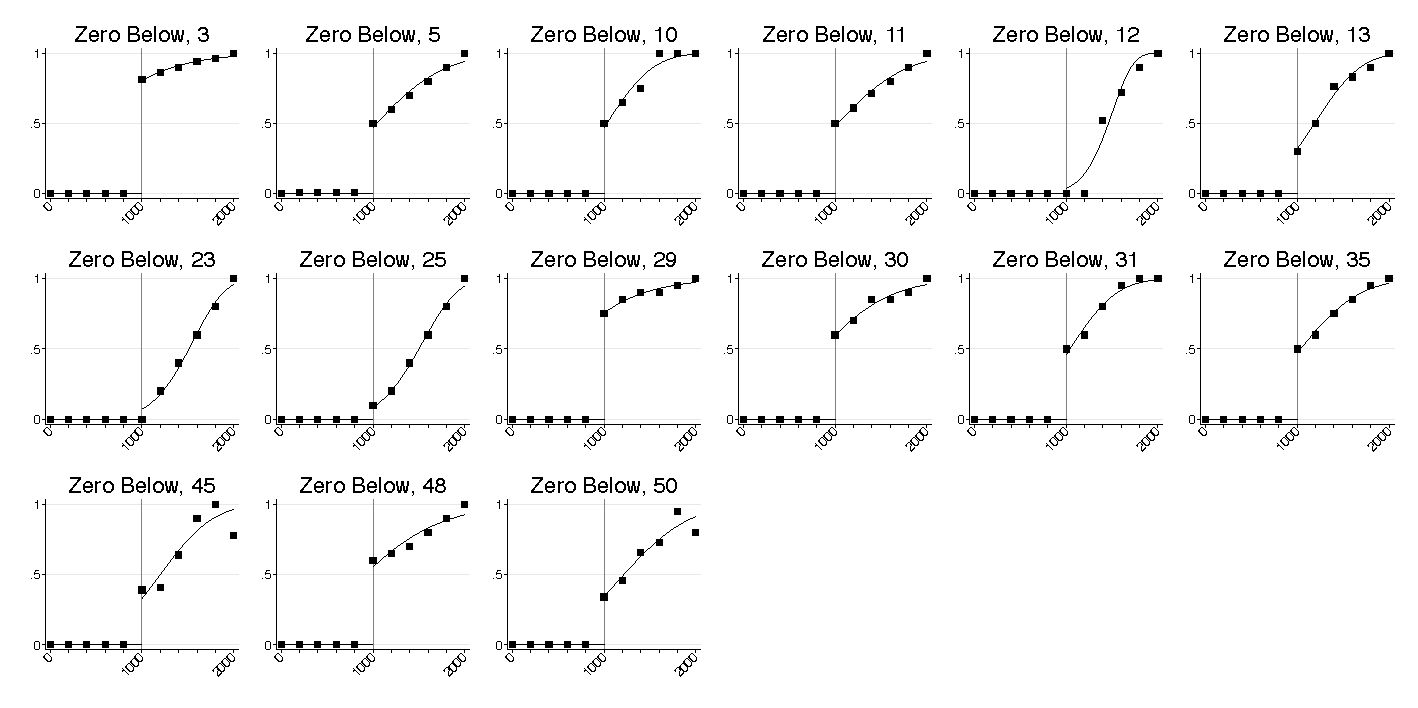
\includegraphics[width=\linewidth]{figures/figure_2.pdf}
   \begin{minipage}{\linewidth}
      \footnotesize
      \textit{The markers show the individual justice rating of endowments with $\{0,200,\ldots,2000\}$ units of living space on a $[0,1]$ scale and the respective JEF of $19$ sufficientarian participants in the global rating task of the Need treatment. The need threshold at $1000$ units is marked by a vertical line.}
   \end{minipage}
   \caption{Sufficientarian individual justice ratings in the global rating task of the Need treatment}\label{fig:figure_2}
\end{figure}

\begin{figure}[h!t!]
   \centering
   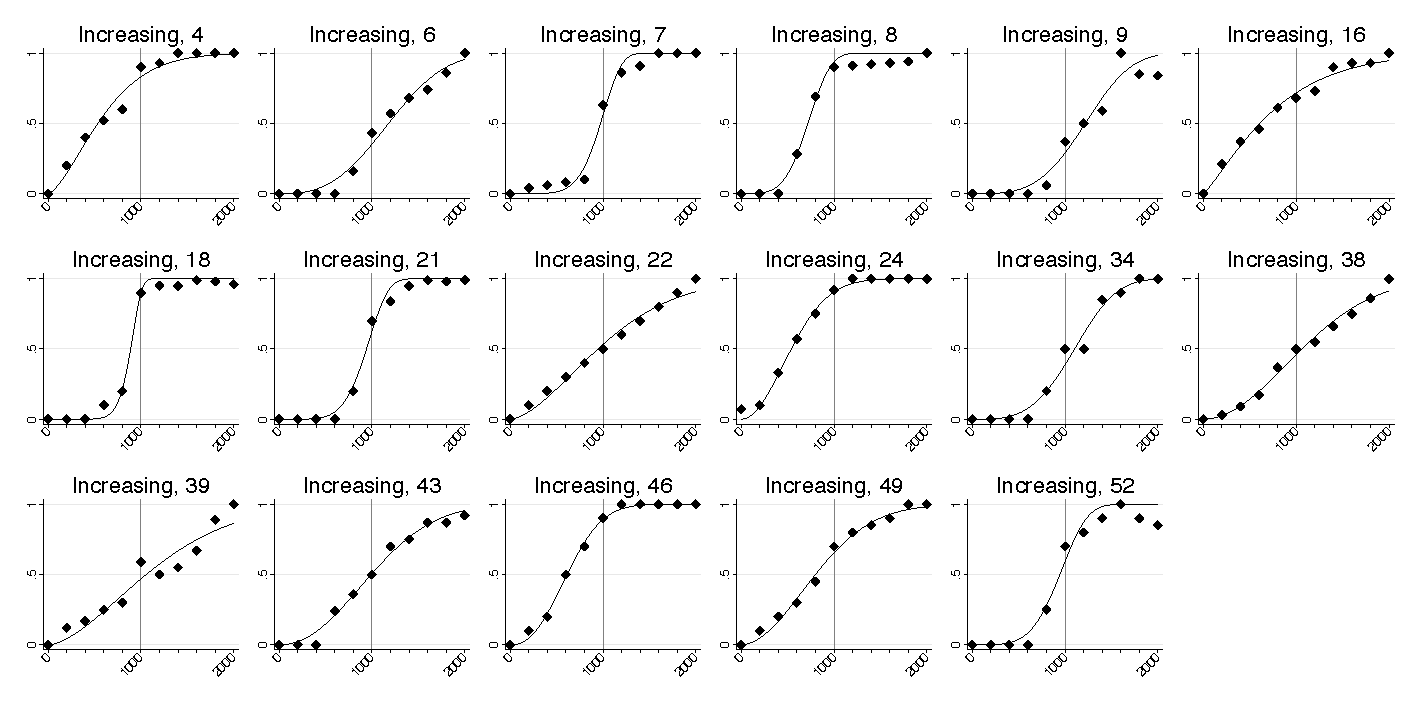
\includegraphics[width=\linewidth]{figures/figure_3.pdf}
   \begin{minipage}{\linewidth}
      \footnotesize
      \textit{The markers show the individual justice rating of endowments with $\{0,200,\ldots,2000\}$ units of living space on a $[0,1]$ scale and the respective JEF of $15$ prioritarian participants in the global rating task of the Need treatment. The need threshold at $1000$ units is marked by a vertical line.}
   \end{minipage}
   \caption{Prioritarian individual justice ratings in the global rating task of the Need treatment}\label{fig:figure_3}
\end{figure}

\begin{figure}[h!t!]
   \centering
   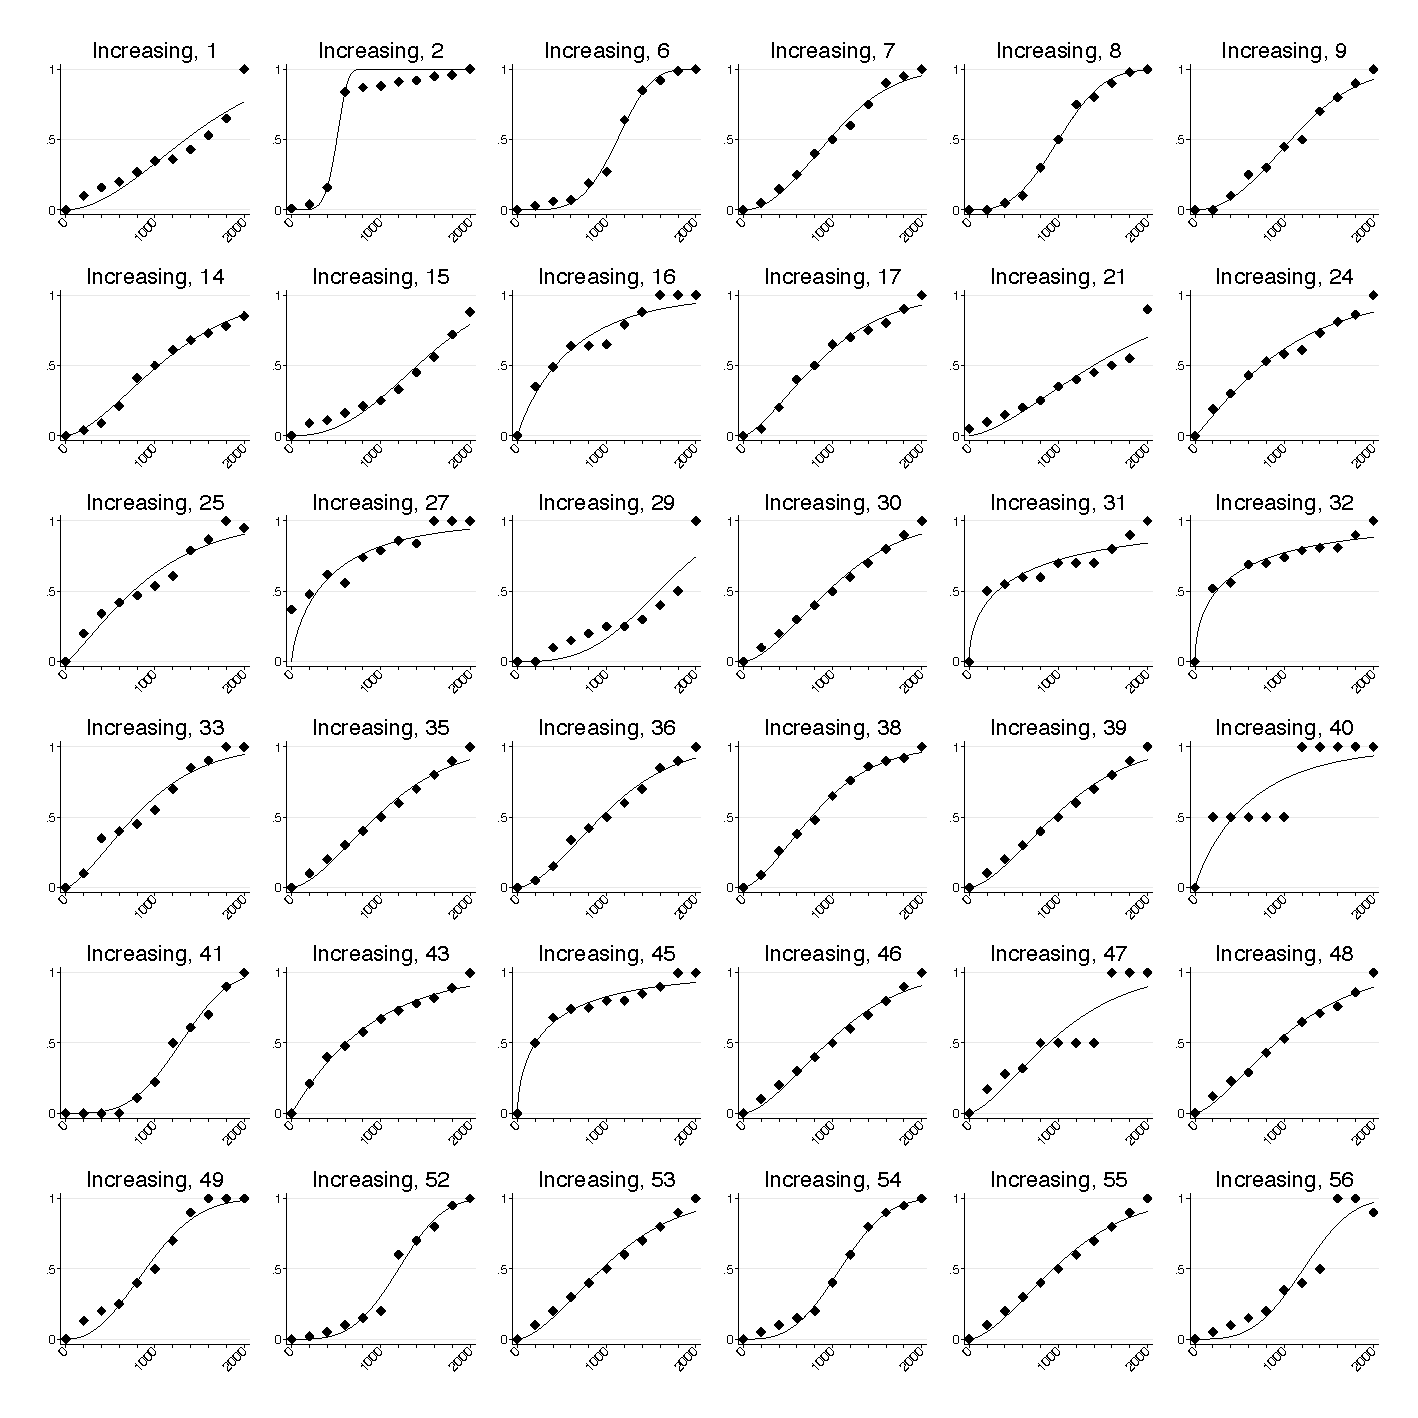
\includegraphics[width=\linewidth]{figures/figure_4.pdf}
   \begin{minipage}{\linewidth}
      \footnotesize
      \textit{The markers show the individual justice rating of endowments with $\{0,200,\ldots,2000\}$ units of living space on a $[0,1]$ scale and the respective JEF of $17$ utilitarian participants in the global rating task of the Need treatment. The need threshold at $1000$ units is marked by a vertical line.}
   \end{minipage}
   \caption{Utilitarian individual justice ratings in the global rating task of the Need treatment}\label{fig:figure_4}
\end{figure}

Figures \ref{fig:figure_2} to \ref{fig:figure_4} show the individual justice ratings (markers) and the estimated JEFs (solid lines) by rating type and subject identification number (ID) in the Need treatment.
Figure \ref{fig:figure_2} collects all subtypes of sufficientarians, Figures \ref{fig:figure_3} and \ref{fig:figure_4} collect prioritarians and utilitarians.
The figures reveal that there is a lot of heterogeneity in regard to the participants' response patterns.
In the Need treatment, there are $8$ participants ($15.4\%$) who exhibit a \textit{hump-shaped} JEF (see Figure \ref{fig:figure_2}).
The hump-shaped JEF reaches its maximum at or slightly above $1000$ units and then drops sharply, suggesting that strict sufficientarians ``punish'' oversupply.
Only $4$ participants ($7.7\%$) exhibit a \textit{binary} JEF that is $0$ (in one case $0.5$) for endowments below and $1$ for endowments at and above the need threshold.
The binary shape of the JEF could be viewed as a qualitative account of sufficientarianism that only distinguishes between unjust insufficient and just sufficient endowments.
The JEFs of $7$ participants ($13.5\%$) increase below and reach the maximum of $1$ at the need threshold.
They are \textit{flat at and above the need threshold}.
This shape of the JEF is compatible with a quantitative account of sufficientarianism that is able to differentiate between different degrees of unjust insufficiency.

$15$ participants ($28.9\%$) rated endowments below the need threshold as completely unfair and only increased their justice ratings at and above the need threshold (see Figure \ref{fig:figure_3}).
A JEF that is \textit{zero below the need threshold} can be interpreted as a strict account of prioritarianism that regards the need threshold as absolute (in this case, undersupply is rated as unconditionally unjust; it might be interpreted as having a \textit{qualitative} aspect; see the differentiation between qualitative and quantitative accounts of need-based justice in Section \ref{sec:principles}).
In demand theory, a similar idea is covered by the Stone-Geary utility function \citep{geary_note_1950,stone_linear_1954}, which assumes that the minimum consumption level is indispensable to life and that only consumption levels exceeding them generate utility.\footnote{For other experimental investigations of need thresholds see, e.\,g., \citet{bauer_winter_2023,bauer_equal_2024}, and, for need thresholds in risky scenarios, \citet{diederich_need_2020}.}
The \textit{utilitarian} type increases her justice rating throughout ($17$ participants, $32.7\%$).
Figure \ref{fig:figure_4} shows slightly different shapes of the JEF, most of which are sigmoid ($k>1$) in the endowment with living space.
In any case, no influence of the information on the need threshold at $1000$ units of living space is visually or formally recognizable here.
Note that we were a bit more generous in this category, including as utilitarian also those $3$ participants whose JEF did not consistently increase (subject numbers $9$, $39$, and $52$).

Overall, in the Need treatment, we find that about one-third of individual justice ratings are compatible with sufficientarianism, priortarianism, and utilitarianism, respectively.\footnote{One subject could not be classified, see Figure \ref{fig:figure_11} in Appendix \ref{sec:app_additional}.}
This means that around two thirds of the participants took the need threshold explicitly into account in their justice ratings.
We looked for differences between the justice types with regard to sociodemographics, living conditions, and political attitudes but found no significant effects.

\begin{figure}[h!t!]
   \centering
   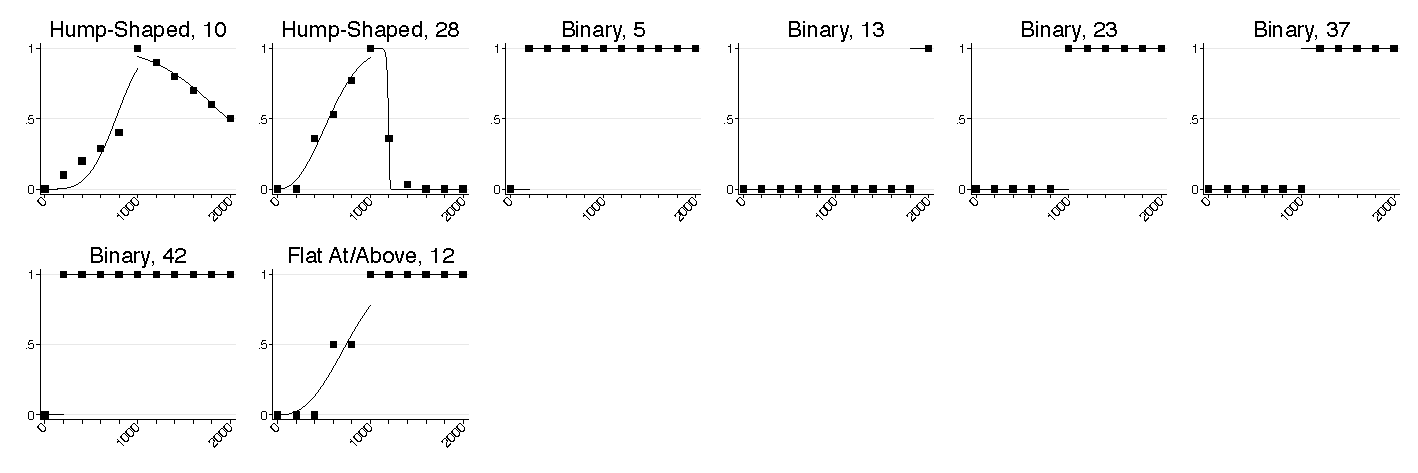
\includegraphics[width=\linewidth]{figures/figure_5.pdf}
   \begin{minipage}{\linewidth}
      \footnotesize
      \textit{The markers show the individual justice rating of endowments with $\{0,200,\ldots,2000\}$ units of living space on a $[0,1]$ scale and the respective JEF of $36$ utilitarian participants in the global rating task of the Need treatment. The need threshold at $1000$ units is marked by a vertical line.}
   \end{minipage}
   \caption{Utilitarian individual justice ratings in the global rating task of the NoNeed treatment}\label{fig:figure_5}
\end{figure}

Analogously, Figures \ref{fig:figure_5} to \ref{fig:figure_7} show the individual justice ratings (markers) and the estimated JEFs (solid lines) by type and subject identification number (ID) in the NoNeed treatment.
The respective column in Table \ref{tab:individual} summarizes the type assignment.
Although there was no communicated need threshold in NoNeed, participants could nevertheless have assumed that people need some minimum endowment with living space in their justice ratings.
In fact, the absolute majority ($36$ participants, $63.2\%$) of the JEFs have a monotonically increasing shape (with a maximum of one non-increasing evaluation being allowed in order to account for errors), so it is clearly \textit{utilitarian}, see Figure \ref{fig:figure_5}.
A proportion test clearly rejects the null hypothesis that Need treatment and NoNeed treatment give rise to the same proportion of utilitarian justice evaluations ($z=3.18$, $p=0.001$).

\begin{figure}[h!t!]
   \centering
   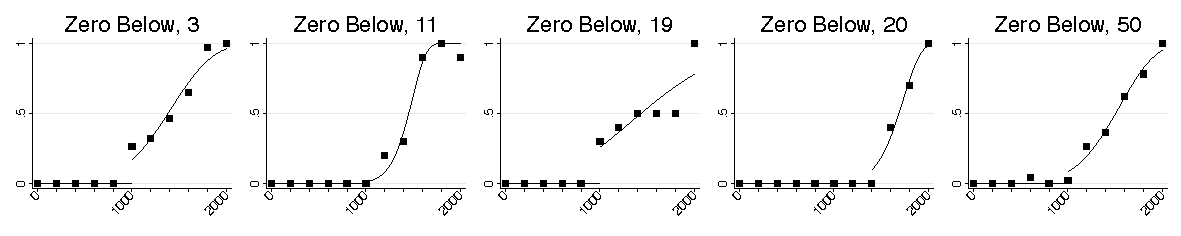
\includegraphics[width=\linewidth]{figures/figure_6.pdf}
   \begin{minipage}{\linewidth}
      \footnotesize
      \textit{The markers show the individual justice rating of endowments with $\{0,200,\ldots,2000\}$ units of living space on a $[0,1]$ scale and the respective JEF of $8$ sufficientarian participants in the global rating task of the Need treatment. The need threshold at $1000$ units is marked by a vertical line.}
   \end{minipage}
   \caption{Sufficientarian individual justice ratings in the global rating task of the NoNeed treatment}\label{fig:figure_6}
\end{figure}

\begin{figure}[h!t!]
   \centering
   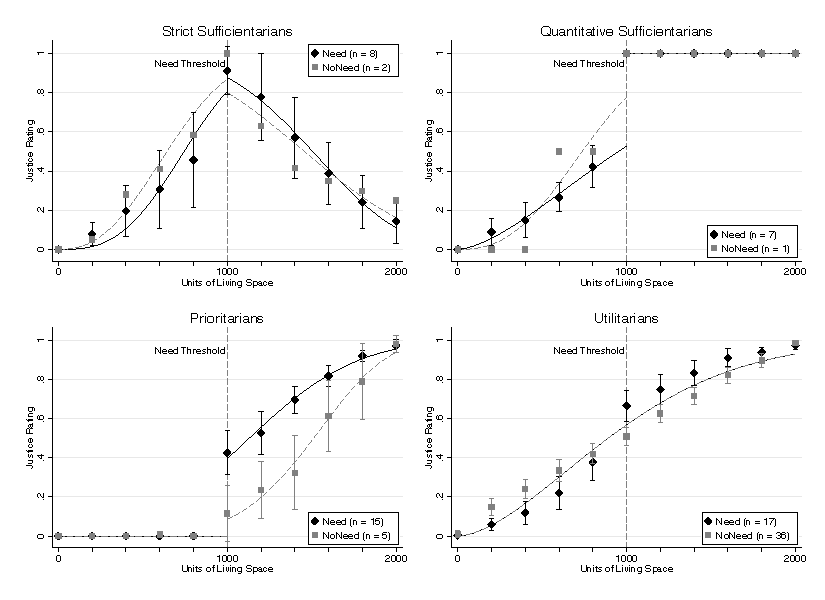
\includegraphics[width=11.7cm]{figures/figure_7.pdf}
   \begin{minipage}{\linewidth}
      \footnotesize
      \textit{The markers show the individual justice rating of endowments with $\{0,200,\ldots,2000\}$ units of living space on a $[0,1]$ scale and the respective JEF of $5$ prioritarian participants in the global rating task of the Need treatment. The need threshold at $1000$ units is marked by a vertical line.}
   \end{minipage}
   \caption{Prioritarian individual justice ratings in the global rating task of the NoNeed treatment}\label{fig:figure_7}
\end{figure}

In NoNeed, we find only two participants with \textit{hump-shaped} JEFs with the maximum justice at $1000$ units of living space, see Figure \ref{fig:figure_6}.
Five participants exhibit a \textit{binary} JEF, which jumps from $0$ to $1$ at some value of units of living space on the interval $[200,1800]$.
A further subject can be classified as quantitative sufficientarian because her JEF is \textit{flat at and above the} (subjective) \textit{need threshold} of 1000.
Altogether, there are $8$ sufficientarian justice evaluations.
A proportion test shows that sufficientarian justice evaluations are almost twice as common among participants in the Need treatment as in the NoNeed treatment ($z=2.72$, $p=0.007$).

There are only $5$ JEFs exhibiting a ``prioritarian'' shape, assuming \textit{zero below} some subjective \textit{need threshold}, see Figure \ref{fig:figure_7}.
Thus, the proportion of prioritarians is almost three times bigger in Need as in NoNeed ($z=2.70$, $p=0.007$).

In NoNeed, we also observe $2$ participants who rated all endowments as perfectly just, which is compatible with a comparative egalitarian justice attitude; $1$ subject rated all endowments as perfectly unjust, which is, perhaps, a ``negative'' egalitarian justice attitude; and $5$ participants stated irregular JEFs, see Figure \ref{fig:figure_12} in Appendix \ref{sec:app_additional}.

To summarize this part of the analysis, it can be stated that the introduction of an explicit need threshold leads to a statistically significant change in the justice evaluation of endowments with living space at the individual level.
The heterogeneity of justice attitudes not only increases with the introduction of the need threshold but also changes in the direction of less utilitarianism and more prioritarianism and sufficientarianism.


%%%%%%%%%%%%%%%%%%%%%%%
% MEAN RATINGS GLOBAL %
%%%%%%%%%%%%%%%%%%%%%%%
\subsection{Mean Justice Ratings in the Global Rating Task}\label{sec:global}
In this subsection, we first take a comparative look at the aggregated JEFs between the two treatments, separately for the five non-comparative justice (sub-)principles.
Thereafter, we aggregate all individual justice ratings into ``social'' JEFs, separately for each treatment.

\begin{figure}[h!t!]
   \centering
   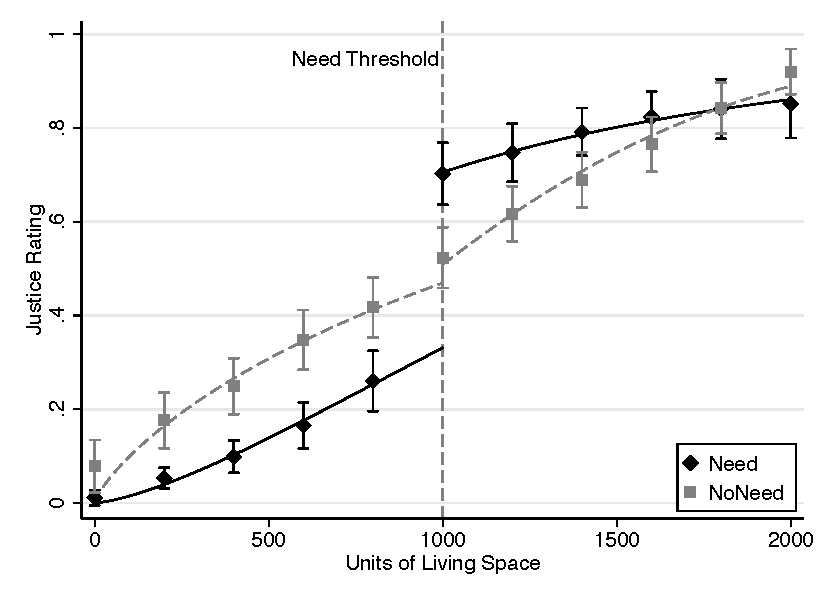
\includegraphics[width=\linewidth]{figures/figure_8.pdf}
   \begin{minipage}{\linewidth}
      \footnotesize
      \textit{The figure shows the mean justice ratings for $x=\{0,200,\ldots,2000\}$ units of living space on a $[0,1]$ scale and the respective $90\%$ confidence intervals in the global rating task of the Need (NoNeed) treatment by justice principle. The solid (dashed) line represents the Weibull fit for the non-constant intervals of the JEF. Qualitative sufficientarians are not included.}
   \end{minipage}
   \caption{Mean justice ratings in the global rating task by justice principle and treatment}
   \label{fig:figure_8}
\end{figure}

Figure \ref{fig:figure_8} shows the mean justice ratings in the global rating task by justice principle and treatment.
The two top panels show the JEFs for strict and quantitative sufficientarians.
Qualitative sufficientarians are not included since their JEF is flat, both below as well as at and above the need threshold.
A statistical comparison between the Need and the NoNeed treatment is hardly possible due to the very small number of cases in the NoNeed treatment.
For strict sufficientarians, neither a two-sided $t$ test nor an exact Wilcoxon rank sum test reject the null hypothesis of equality of the mean justice ratings for the individual endowments from $0$ to $2000$ units (for case numbers, means, standard errors, test results, and parameter estimates, see Table \ref{tab:global_ratings_principle} in Appendix \ref{sec:app_additional}).
We estimated the shape parameter $k$ of the JEF separately for the ratings below and above the need threshold.
In Need, the shape parameters are significantly greater than $1$, implying that the JEF is sigmoid below and above the need threshold.
In NoNeed, the shape parameters are also greater than $1$, but we do not have enough observations to obtain significant results.
For quantitative sufficientarians, we estimated the JEF only for the interval $[0,1000)$, because it is flat at and above the need threshold by definition.
In the Need treatment, the shape parameter of $1.59$ shows a sigmoid shape of the JEF ($k$ is weakly significantly greater than $1$, $p=0.090$).

The prioritarians' JEFs are shown in the bottom left panel of Figure \ref{fig:figure_8}.
Here, the JEF is flat on the interval $[0,1000)$ by definition.\footnote{We ignore small deviations from zero, which are probably due to participants' inaccuracies in the slider settings.}
We fitted the Weibull distribution to the justice ratings of $[1000,2000]$ units of living space.
For each endowment stimulus between $1000$ and $1600$ units, the mean justice rating in the Need treatment is significantly greater than in the NoNeed treatment, both according to $t$ tests and exact Wilcoxon rank sum tests (the $t$ test rejects the null hypothesis of equality of the means also for $1800$ units, see Table \ref{tab:global_ratings_principle} in Appendix \ref{sec:app_additional}).
In both treatments, the JEF is sigmoid according to the shape parameter.
In the Need treatment, however, the inflection point is already at $1083$ units, while it is at $1555$ units in NoNeed.\footnote{We derived the inflection points by taking the second derivatives of the JEFs and setting them equal to zero. The corresponding Maple outputs are available from the authors on request.}
Hence, the JEF of the prioritarians treated with a need threshold shows a largely concave shape above the need threshold, so that after the ``jump'' at $1000$ units additional living space contributes less and less to greater justice.

In the bottom right panel of Figure \ref{fig:figure_8}, we compare the utilitarians' mean justice ratings and JEFs.
Here, the mean justice ratings in the Need treatment are significantly lower for $200$, $400$, and $600$ units of living space and significantly higher for $1000$ to $1600$ units of living space than in the NoNeed treatment (the respective $t$ tests and exact Wilcoxon rank sum tests are each significant at least at the $10\%$ level, see Table \ref{tab:global_ratings_principle} in Appendix \ref{sec:app_additional}).
Both JEFs are sigmoid according to the shape parameter.
However, the curvature of the Need JEF is significantly greater than the NoNeed JEF and the inflection points are at $801$ units and $529$ units, respectively.
Thus, the need threshold not only causes low endowments to be rated as less just and higher endowments as more just, but also increasing marginal justice evaluations below and decreasing marginal justice evaluations above the need threshold.

The comparison between the two treatments thus shows not only the shift away from utilitarian towards sufficientarian and prioritarian evaluations of justice, as demonstrated in the previous subsection, but also a higher rating of endowments above the need threshold among prioritarians and among the shrinking group of utilitarians, as well as a lower rating of lower endowments among utilitarians.
This means that even the utilitarian evaluations of justice take needs into account.

Figure \ref{fig:figure_9} shows the participants' mean justice ratings aggregated across all five justice (sub-)principles in the global rating task by treatment and endowment.
The respective means, standard errors, and $t$ tests are stated in Table \ref{tab:global_ratings_full}.
In a first step, we fit the Weibull distribution to the data without assuming a reference point ($r=0$).
Then, we checked for each $r\in\{200,400,\ldots,2000\}$ whether the fit in terms of the adjusted coefficient of determination $\bar{R}^2$ and the root mean square error ($RMSE$) improved when interacting the parameters of the Weibull distribution ($\lambda$, $k$) with a dummy variable $D=0$ for $x<0$ and $D=1$ for $x\ge0$ units of living space.
Table \ref{tab:goodness} in Appendix \ref{sec:app_additional} shows that, in both treatments, the best fit was obtained by setting the reference point to $1000$ units.
In the Need treatment, the reference point corresponds to the need threshold as expected.
In the NoNeed treatment, there was no explicit need threshold, but, as we have shown in Subsection \ref{sec:individual}, some participants nevertheless oriented themselves towards this value, so that they could be classified as sufficientarians or prioritarians.\footnote{Since it could be objected that the reference point at $1000$ units is mainly due to the strict sufficientarians whose JEFs are hump-shaped, we conducted the entire analysis with a conditional sample containing only the $42$ (Need) and $51$ (NoNeed) participants who exhibit weakly monotonically increasing justice ratings. In addition to the $8$ ($2$) strict sufficientarians, we also dropped $4$ participants with constant or irregular ratings from the sample in NoNeed. Appendices \ref{sec:app_conditional_absolute} and \ref{sec:app_conditional_relative} provide the respective tables and figures. The analysis with the conditional sample provides qualitatively and quantitatively comparable results to the analysis with the complete sample.}
Hence, the regression table also displays the Weibull fit for $r=1000$.
The figure shows only the JEFs with reference point.
The dashed line represents the Weibull fit for NoNeed and the solid line for Need.

\begin{figure}[ht!]
   \centering
   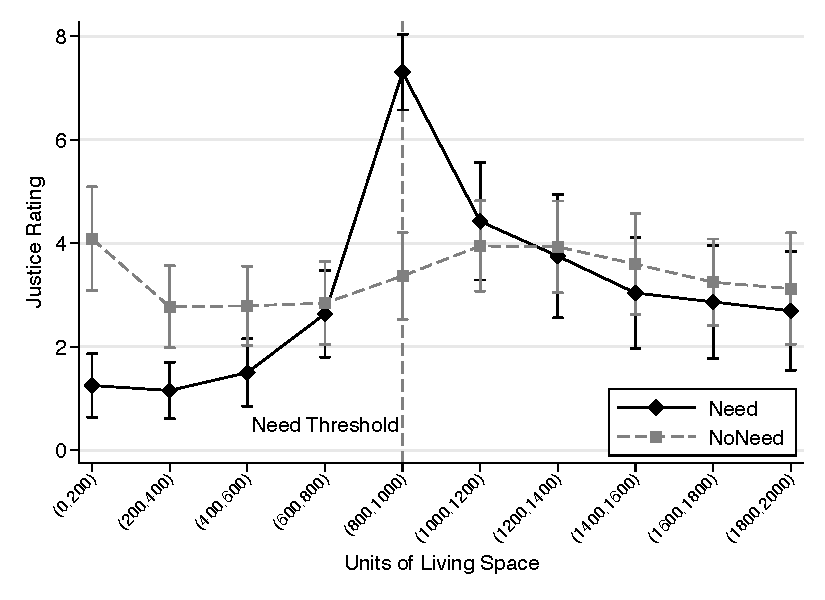
\includegraphics{figures/figure_9.pdf}
   \begin{minipage}{\linewidth}
      \footnotesize
      \textit{The figure shows the mean justice ratings for $x=\{0,200,\ldots,2000\}$ units of living space on a $[0,1]$ scale and the respective $90\%$ confidence intervals of $n=52$ ($n=57$) participants in the global rating task of the Need (NoNeed) treatment. The solid (dashed) line represents the Weibull fit with $r=1000$ as reference point.}
   \end{minipage}
   \caption{Mean justice ratings in the global rating task}
   \label{fig:figure_9}
\end{figure}

\begin{table}[ht!]
   \centering
   \caption{Mean justice ratings in the global rating task by treatment}\label{tab:global_ratings_full}
   \begin{tabular}{rd{1.3}d{1.3}cd{1.3}d{1.3}cd{2.3}d{1.3}d{1.3}}                         \\[-0.5ex]\hline
           & \multicolumn{2}{c}{Need}                              &   & \multicolumn{2}{c}{NoNeed}                            &   & \multicolumn{3}{c}{$t$ Test}                                                                  \\\cline{2-3}\cline{5-6}\cline{8-10}
   Units   & \multicolumn{1}{c}{Mean}   & \multicolumn{1}{c}{SE}   &   & \multicolumn{1}{c}{Mean}   & \multicolumn{1}{c}{SE}   &   & \multicolumn{1}{c}{Mean Diff.}   & \multicolumn{1}{c}{SE}   & \multicolumn{1}{c}{$p$}         \\\hline\hline
      0    & 0.011                      & 0.009                    &   & 0.078                      & 0.034                    &   & -0.067                           & 0.036                    & 0.070                           \\
    200    & 0.053                      & 0.013                    &   & 0.176                      & 0.036                    &   & -0.123                           & 0.039                    & 0.002                           \\
    400    & 0.099                      & 0.021                    &   & 0.249                      & 0.036                    &   & -0.150                           & 0.042                    & 0.000                           \\
    600    & 0.165                      & 0.029                    &   & 0.348                      & 0.038                    &   & -0.182                           & 0.049                    & 0.000                           \\
    800    & 0.260                      & 0.038                    &   & 0.417                      & 0.038                    &   & -0.157                           & 0.054                    & 0.005                           \\\hline
   1000    & 0.702                      & 0.040                    &   & 0.523                      & 0.039                    &   &  0.179                           & 0.055                    & 0.002                           \\
   1200    & 0.747                      & 0.037                    &   & 0.617                      & 0.035                    &   &  0.130                           & 0.051                    & 0.012                           \\
   1400    & 0.792                      & 0.030                    &   & 0.689                      & 0.035                    &   &  0.102                           & 0.047                    & 0.032                           \\
   1600    & 0.824                      & 0.032                    &   & 0.765                      & 0.035                    &   &  0.059                           & 0.048                    & 0.223                           \\
   1800    & 0.840                      & 0.038                    &   & 0.842                      & 0.032                    &   & -0.002                           & 0.050                    & 0.973                           \\
   2000    & 0.852                      & 0.044                    &   & 0.920                      & 0.029                    &   & -0.068                           & 0.051                    & 0.186                           \\\hline
   \multicolumn{10}{p{13cm}}{\footnotesize\textit{The table shows the mean justice ratings of $x=\{0,200,\ldots,2000\}$ units of living space on a $[0,1]$ scale and the respective standard errors of $n=52$ ($n=57$) participants in the global rating task of the Need (NoNeed) treatment, and the results of a $t$ test (mean differences, standard errors, $p$ values) on the mean difference (Welch test). Positive (negative) mean differences indicate that the respective number of units of living space was rated as more (less) just in the Need treatment than in the NoNeed treatment.}}
   \end{tabular}
\end{table}

\begin{table}[ht!]
   \centering
   \caption{Fitted parameters of the Weibull distribution}\label{tab:weibull_full}
   \begin{tabular}{ld{2.6}d{3.6}cd{2.6}d{3.6}}                                                                                                               \\[-0.5ex]\hline
                           & \multicolumn{2}{c}{Need}                                     &   & \multicolumn{2}{c}{NoNeed}                                   \\\cline{2-3}\cline{5-6}
   Parameter               & \multicolumn{1}{c}{$r=0$}   & \multicolumn{1}{c}{$r=1000$}   &   & \multicolumn{1}{c}{$r=0$}   & \multicolumn{1}{c}{$r=1000$}   \\\hline\hline
   $\lambda_0$             &   0.00087^{***}             &   0.00053^{***}                &   &   0.00084^{***}             &   0.00056^{***}                \\
                           &  (0.00002)                  &  (0.00016)                     &   &  (0.00002)                  &  (0.00015)                     \\
   $\lambda_1\times D$     &                             &   0.00081^{***}                &   &                             &   0.00025^{*}                  \\
                           &                             &  (0.00027)                     &   &                             &  (0.00015)                     \\
   $k_0$                   &   2.00423^{***}             &   1.43208^{***}                &   &   1.25965^{***}             &   0.78351^{***}                \\
                           &  (0.12243)                  &  (0.39590)                     &   &  (0.08312)                  &  (0.17109)                     \\[0.5ex]
   H0: $p(k_0\le 1)$       &   0.000                     &   0.138                        &   &   0.001                     &   0.897                        \\[0.5ex]
   $k_1\times D$           &                             &  -0.74159^{*}                  &   &                             &   0.84806^{***}                \\
                           &                             &  (0.43163)                     &   &                             &  (0.26140)                     \\[0.5ex] 
   H0: $p(k_0+k_1\le 1)$   &                             &   0.964                        &   &                             &   0.001                        \\[0.5ex]\hline
   $n$                     & 572                         & 572                            &   & 627                         & 627                            \\
   $\bar{R}^2$             &   0.8542                    &   0.8704                       &   &   0.8220                    &   0.8242                       \\
   $RMSE$                  &   0.2434                    &   0.2296                       &   &   0.2678                    &   0.2661                       \\\hline
   \multicolumn{6}{p{13cm}}{\footnotesize\textit{The table shows the results of fitting a Weibull distribution to the participants' justice ratings in the global rating task using nonlinear OLS by treatment. $D=0\,(1)$ for $x<(\ge)1000$ units of living space. First row: means, second row: standard errors. Significance levels: $^{*}p\le0.10$, $^{**}p\le0.05$, $^{***}p\le0.01$.}}
   \end{tabular}
\end{table}

Figure \ref{fig:figure_9} suggests that the mean justice ratings in the NoNeed treatment initially increase with decreasing rate.
At $r=1000$ units, there is a small ``jump'', although no reference point was given.
The ``jump'' indicates that at least some participants perceived $1000$ units of living space---which is half the maximum possible---as some kind of natural reference point, giving rise to sufficientarian or prioritarian justice preferences.
For endowments of at least $1000$ units, the mean justice rating increases again at a decreasing rate.
According to the Weibull regression in Table \ref{tab:weibull_full} (NoNeed, $r=1000$), we cannot reject the null hypothesis of concavity ($k_0\le 1$) for endowments with living space smaller than $1000$ units.
For endowments at and above $1000$ units, the null hypothesis ($k_0+k_1\le 1$) is rejected.
However, the inflection point is at $690$ units, i.\,e., below the relevant range of $[1000,2000]$.\footnote{The Maple output for computing the derivatives of $J(c)$ is available from the authors on request.}
Overall, in the NoNeed treatment, the JEF consists of two concave segments.

Turning to the Need treatment, the solid line in Figure \ref{fig:figure_9} exhibits a convex shape below, a ``jump'' of about $35$ percentage points at, and a concave shape above the need threshold.
The inflection point is at $817$ units of living space, this is just below the need threshold.
However, according to Table \ref{tab:weibull_full} (NoNeed, $r=1000$), the null hypothesis of concavity for endowments with living space smaller than $1000$ units is just barely not rejected ($p=0.138$).
For endowments in the range $[1000,2000]$, concavity is clearly not rejected ($p=0.964$).
Overall, in the Need treatment, the JEF tends to be convex below the need threshold and is concave above.

Thus, Figure \ref{fig:figure_9} displays a striking difference between the Need and the NoNeed treatment.
According to Table \ref{tab:global_ratings_full}, mean justice ratings are significantly lower (higher) in the Need than in the NoNeed treatment (except for $0$ and for $1600$ or more units of living space).


%%%%%%%%%%%%%%%%%%%%%%%%%
% MEAN RATINGS RELATIVE %
%%%%%%%%%%%%%%%%%%%%%%%%%
\subsection{Mean Justice Ratings in the Relative Rating Task}\label{sec:relative}
As noted in Subsection \ref{sec:treatments}, we conducted the relative rating task in order to address the concern that bunching at extreme values may bias participants' justice ratings in the absolute rating task.
Again, we use the full sample.
In Appendix \ref{sec:app_conditional_relative}, we show the results for the conditional sample, only including participants who exhibit weakly monotonically increasing justice ratings.

Figure \ref{fig:figure_10} depicts the results of the relative rating task, which provided participants for every pair-wise comparison with a separate rating scale.
Means, standard errors and $t$ tests are stated in Table \ref{tab:relative_ratings_full}.

\begin{figure}[h]
   \centering
   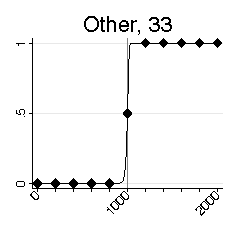
\includegraphics{figures/figure_10.pdf}
   \begin{minipage}{\linewidth}
      \footnotesize
      \textit{The figure shows the mean justice ratings of comparing two adjacent endowments with $\{(0,200),(200,400),\ldots,(1800,2000)\}$ units of living space on a $[-11,+11]$ Likert scale and the respective $90\%$ confidence intervals of $n=52$ ($n=57$) participants in the relative rating task of the Need (NoNeed) treatment. Positive (negative) numbers indicate that the larger endowment was rated as more (less) just than the smaller endowment.}
   \end{minipage}
   \caption{Mean justice ratings in the relative rating task}
   \label{fig:figure_10}
\end{figure}

\begin{table}[ht!]
   \centering
   \caption{Mean justice ratings in the relative rating task by treatment}\label{tab:relative_ratings_full}
   \begin{tabular}{ld{1.2}d{1.2}cd{1.2}d{1.2}cd{1.2}d{1.2}d{1.2}}                           \\[-0.5ex]\hline
                   & \multicolumn{2}{c}{Need}                              &   & \multicolumn{2}{c}{NoNeed}                            &   & \multicolumn{3}{c}{$t$ Test}                                                             \\\cline{2-3}\cline{5-6}\cline{8-10}
   Units           & \multicolumn{1}{c}{Mean}   & \multicolumn{1}{c}{SE}   &   & \multicolumn{1}{c}{Mean}   & \multicolumn{1}{c}{SE}   &   & \multicolumn{1}{c}{Mean Diff.}   & \multicolumn{1}{c}{SE}   & \multicolumn{1}{c}{$p$}         \\\hline\hline
      $(0,200)$    & 1.25                       & 0.37                     &   & 4.09                       & 0.60                     &   & -2.84                            & 0.72                     & 0.000                           \\
    $(200,400)$    & 1.15                       & 0.33                     &   & 2.77                       & 0.47                     &   & -1.62                            & 0.58                     & 0.007                           \\
    $(400,600)$    & 1.50                       & 0.39                     &   & 2.79                       & 0.46                     &   & -1.29                            & 0.61                     & 0.036                           \\
    $(600,800)$    & 2.63                       & 0.50                     &   & 2.84                       & 0.48                     &   & -0.21                            & 0.69                     & 0.765                           \\
    $(800,1000)$   & 7.31                       & 0.44                     &   & 3.37                       & 0.50                     &   &  3.94                            & 0.67                     & 0.000                           \\\hline
   $(1000,1200)$   & 4.42                       & 0.68                     &   & 3.95                       & 0.52                     &   &  0.48                            & 0.85                     & 0.576                           \\
   $(1200,1400)$   & 3.75                       & 0.71                     &   & 3.93                       & 0.53                     &   & -0.18                            & 0.88                     & 0.838                           \\
   $(1400,1600)$   & 3.04                       & 0.64                     &   & 3.60                       & 0.58                     &   & -0.56                            & 0.88                     & 0.518                           \\
   $(1600,1800)$   & 2.87                       & 0.65                     &   & 3.24                       & 0.50                     &   & -0.38                            & 0.81                     & 0.641                           \\
   $(1800,2000)$   & 2.69                       & 0.69                     &   & 3.12                       & 0.64                     &   & -0.43                            & 0.94                     & 0.648                           \\\hline
   \multicolumn{10}{p{13cm}}{\footnotesize\textit{The table shows the mean justice ratings comparing two adjacent endowments with $\{(0,200),(200,400),\ldots,(1800,2000)\}$ units of living space on a $[-11,+11]$ Likert scale of $n=52$ ($n=57$) participants in the relative rating task of the Need (NoNeed) treatment, and the results of a $t$ test (mean differences, standard errors, $p$ values) on the mean difference (Welch test). Positive (negative) means indicate that the larger endowment was rated as more (less) just than the smaller endowment. Positive (negative) mean differences indicate that the respective comparison was rated as more (less) just in the Need treatment than in the NoNeed treatment.}}
   \end{tabular}
\end{table}

On the whole, Figure \ref{fig:figure_10} corroborates the results of the absolute rating task.
In the Need treatment, increasing the endowment by $200$ units of living space raises justice ratings only by about $1$ to $2$ points on the Likert scale when the adjustment takes place below the need threshold; it raises justice ratings by about $3$ to $5$ points when above the need threshold; and justice ratings ``jump'' by $7$ points when the need threshold is met exactly.

Relative justice ratings are significantly worse in the Need treatment than in the NoNeed treatment for adjustments below the need threshold (with the exception of ($600,800$) which is insignificant) and better for ($800,1000$); they are identical for adjustments above the need threshold.

In the NoNeed treatment, relative justice ratings meander between slightly below $3$ and above $4$ points.
The drop from $4.09$ ($0,200$) to $2.77$ ($200,400$) points in the beginning is significant ($p\le 0.01$, two-tailed $t$ test), which supports concavity of the JEF for low endowments in the NoNeed treatment.
Using the full instead of the conditional sample does not change the results (see Figure \ref{fig:figure_14} and Table \ref{tab:relative_ratings_conditional} in Appendix \ref{sec:app_conditional_relative}).


%%%%%%%%%%%%%%
% CONCLUSION %
%%%%%%%%%%%%%%
\section{Conclusion}\label{sec:conclusion}
While the public and scientific debate about justice is often dominated by comparative notions, such as egalitarianism, we have turned to non-comparative judgments of justice in this paper.
To shed light on the question of what role need satisfaction plays in non-comparative justice ratings concerning endowments with goods, we used a vignette experiment to examine laypeople's justice ratings.

Participants were asked to imagine a fictitious world in which it is the responsibility of the state to provide housing.
We presented participants with a series of scenarios in each of which the state decided to build a different amount of housing (ranging from $0$ to $2000$ fictitious units of living space).
To exclude the comparative dimension, all households are endowed with the same amount of living space.
In one treatment (Need), participants were informed that residents of the region consider a specific amount of living space ($1000$ fictitious units of living space) as necessary for a decent life.
The amount needed is the same for all households to, again, exclude comparative considerations.
Consequently, with their knowledge of the need threshold, participants had to make a non-comparative judgment about the justice of the ``representative'' household's endowment with living space.
In a control group (NoNeed), no such threshold was mentioned.

Participants ($n=109$) were recruited by the WISO experimental laboratory at the University of Hamburg, where the experiment took place.
Every participant was randomly assigned to the Need or the NoNeed treatment.
Then, they were given two different tasks.
In the global rating task, they had to rate the justice of the $11$ scenarios separately on a scale from $0$ to $100\%$, with $100\%$ representing a ``perfectly just'' distribution of living space.
In the relative rating task, they had to evaluate the difference in justice between two adjacent scenarios on an $11$-point Likert scale, with $1$ representing that both scenarios are ``equally just/unjust'' and $11$ representing that one scenario is ``much more just'' than the other.

Using this setup, we find that on an individual level, there is a very heterogeneous picture of different principles of justice.
About one third of the participants could be assigned to sufficientarianism, prioritarianism, and utilitarianism, respectively.
For sufficientarians, it is perfectly just if the representative household receives exactly the amount of housing it needs.
However, we have identified three subtypes: Strict sufficientarians exhibit a hump-shaped justice evaluation function (JEF), so they would prefer the household to be provided with the exact living space needed rather than building even more living space.
Qualitative sufficientarians completely reject all endowments below the need threshold and equally prefer all endowments that at least meet the need, while quantitative sufficientarians also distinguish between differently unjust endowments that do not meet the need.
Like qualitative sufficientarians, prioritarians perceive endowments that do not meet the need of the households as completely unjust.
However, in contrast to sufficientarianism, prioritarianism means that above the need threshold, the justice rating increases with increasing endowment with living space.
Irrespective of the need threshold, the utilitarians feel that every increase in the provision of living space is beneficial and, therefore, increases justice.
Interestingly enough, the Need treatment significantly shifts justice ratings in favor of sufficientariansm and prioritarianism.
But even among utilitarians, the introduction of a need threshold leads to a significantly lower justice rating of low endowments and a significantly better justice rating of higher endowments.

The analysis of the mean justice ratings in the global rating task shows that the introduction of the need threshold leads to a sharp ``jump'' in the justice ratings at the need threshold and to a JEF that tends to be sigmoid.
The JEF is convex below the need threshold and concave above it, so that the average justice ratings for smaller endowments are lower and higher for higher endowments than without the need threshold.
This pattern is also confirmed by the results of the relative rating task.

The need threshold can, therefore, be seen as an important reference point for the individual and ``social'' justice evaluation of goods.
The role of such reference points for judgment and decision making in both risk-free and risky contexts is well documented \citep{kuhberger_influence_1998,kuhberger_choice_2013}.
In this sense, the information about the household's need can be understood as an external framing that divides the set of endowments with living space into gains (above the need threshold) and losses (below the need threshold).
This can also explain, at least in part, the sigmoid form of the aggregated JEF, analogous to the value function of Prospect Theory which is also convex below and concave above the reference point \citep{kahneman_prospect_1979}.
However, the aggregate JEF differs from the value function of Prospect Theory in many ways: The JEF is bounded, while the value function is unbounded; there is a ``jump'' in the justice valuation at the reference point, while the value function has a ``kink''; and the framing affects the curvature of the JEF, while the value function has different slopes for gains and losses (loss aversion) \citep{tversky_loss_1991}.\footnote{Convexity of the value function for losses and concavity for gains is called the ``reflection effect'' and is usually associated with a risky choice setting, i.\,e., risk seeking for losses and risk avoidance for gains.} However, as \citet{trueblood_reference_2015} showed in a perception task, the reference point effect on the valuation of consumer goods also exists without loss aversion.

At the beginning of our study, following \citet{frankfurt_inequality_2015} and \citet{miller_principles_1999}, we defined need-based justice as a person having to have enough to lead a decent life.
With sufficientarianism, prioritarianism, and utilitarianism, we have found three theoretically and empirically convincing non-comparative principles for the justice rating of endowments with goods, given a household's need.
However, political actors and other stakeholders could use the dependency of the applied principles of justice and the shape of the justice evaluation function on the external framing in line with their own objectives in order to create a mood for or against the provision of goods.

It should not go unmentioned that our study also has some limitations.
First of all, an experimental study with a small number of student participants is not representative of the population as a whole.
The vignettes depicted hypothetical situations and there were no financial or other real-life consequences of making ``good'' or ``bad'' decisions.
Furthermore, the analysis only covers non-comparative fairness judgments and disregards efficiency considerations, although comparisons and trade-offs between fairness and efficiency certainly play a role in the real world.
Finally, it would be interesting to see whether other reference points, such as an average or a desired endowment with living space, have similar effects on justice evaluations as the introduction of a need threshold.
We leave the clarification of these questions to further research.


%%%%%%%%%%%%%%%%
% DECLARATIONS %
%%%%%%%%%%%%%%%%
\section*{Declarations}\label{sec:declarations}

\subsection*{Ethical Approval}
Since this study is an anonymous standard survey utilizing hypothetical vignettes and assessing uncritical opinions, no additional approval was sought from an ethics commission.

\subsection*{Competing interests}
The authors declare no competing interests.

\subsection*{Authors' contributions}
All authors contributed equally to this work.

\subsection*{Funding}
Financial support by the German Research Foundation (DFG Grants SI $1731/2-2$, TR $458/6-2$) is gratefully acknowledged.

\subsection*{Availability of data and materials}
Data and do files for analysis with Stata are available from \url{https://github.com/alephmembeth/need-reference-point}.


%%%%%%%%%%%%%%%%
% BIBLIOGRAPHY %
%%%%%%%%%%%%%%%%
\newpage
\bibliography{references.bib}


%%%%%%%%%%%%%%%%%%%%
% ACKNOWLEDGEMENTS %
%%%%%%%%%%%%%%%%%%%%
\section*{Acknowledgements}
We are indebted to the support and input throughout all project phases by Jan Romann, Nils Springhorn, and Mark Siebel.
Moreover, we thank James Konow, Jakob Koscholke, Michael Schippers, Thomas Schramme, and Kai Spiekermann, as well as participants at DFG Research Group 2104 meetings for helpful discussions.
We would also like to thank Abigail Burleigh for her thorough proofreading of the manuscript.


%%%%%%%%%%%%
% APPENDIX %
%%%%%%%%%%%%
\newpage
\appendix


%%%%%%%%%%%%%%%%%%%%%%%%%%%%%%%%%%%%%
% MEAN RATINGS GLOBAL (CONDITIONAL) %
%%%%%%%%%%%%%%%%%%%%%%%%%%%%%%%%%%%%%
\section{Additional Figures and Tables}\label{sec:app_additional}
\begin{figure}[hb]
   \centering
   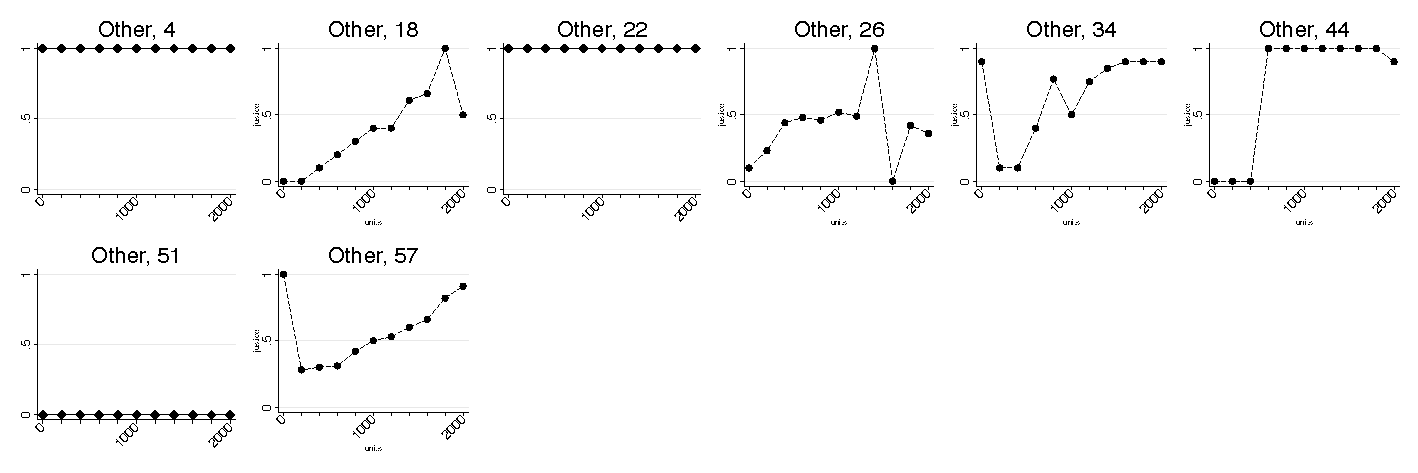
\includegraphics[width=4cm]{figures/figure_11.pdf}
   \begin{minipage}{\linewidth}
      \footnotesize
      \textit{The markers show the individual justice rating of endowments with $\{0,200,\ldots,2000\}$ units of living space on a $[0,1]$ scale and the respective JEF of $1$ other subject in the global rating task of the Need treatment. The need threshold at $1000$ units is marked by a vertical line.}
   \end{minipage}
   \caption{Other individual justice ratings in the global rating task of the Need treatment}\label{fig:figure_11}
\end{figure}

\begin{figure}[hb]
   \centering
   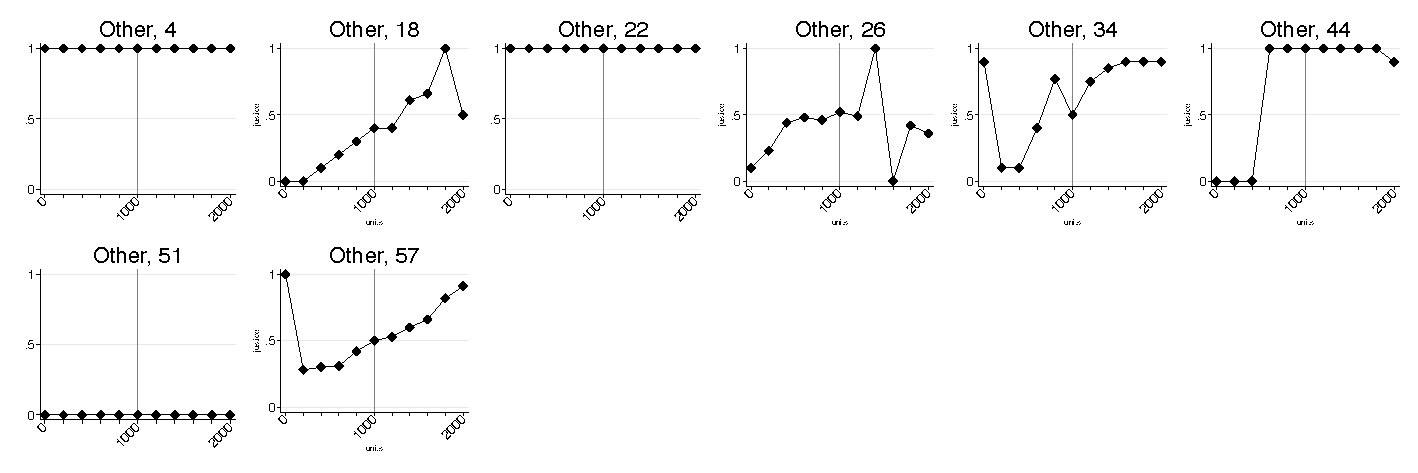
\includegraphics[width=\linewidth]{figures/figure_12.pdf}
   \begin{minipage}{\linewidth}
      \footnotesize
      \textit{The markers show the individual justice rating of endowments with $\{0,200,\ldots,2000\}$ units of living space on a $[0,1]$ scale and the respective JEF of $8$ other participants in the global rating task of the Need treatment. The need threshold at $1000$ units is marked by a vertical line.}
   \end{minipage}
   \caption{Other individual justice ratings in the global rating task of the NoNeed treatment}\label{fig:figure_12}
\end{figure}

\clearpage
\begin{landscape}
   \begin{table}[h!t!]
      \centering
      \caption{Mean justice ratings in the global rating task by justice principle and treatment}\label{tab:global_ratings_principle}
      {\footnotesize
         \begin{tabular}{rrrrrrrrrrrrr}\hline
                          & \multicolumn{3}{c}{Strict}             & \multicolumn{3}{c}{Quantitative}                                                                                                    \\
                          & \multicolumn{3}{c}{Sufficientarians}   & \multicolumn{3}{c}{Sufficientarians}   & \multicolumn{3}{c}{Prioritarians } & \multicolumn{3}{c}{Utilitarians }                     \\\cline{2-13}
            Units         & Need            & NoNeed    & $p$      & Need            & NoNeed    & $p$      & Need            & NoNeed           & $p$     & Need            & NoNeed          & $p$     \\\hline\hline
            $n$           &  8              &  2        &          &  7              &  1        &          & 15              &  5               &         & 17              & 36              &         \\\hline
               0          &  0              &  0        & ---      &  0              &  0        & ---      &  0              &  0               & ---     &  0.004          &  0.012          & 0.613   \\
                          & (0.000)         & (0.000)   & ---      & (0.000)         & (0.000)   & ---      & (0.000)         & (0.000)          & ---     & (0.004)         & (0.010)         & 1.000   \\
             200          &  0.079          &  0.050    & 0.645    &  0.089          &  0        & 0.059    &  0              &  0               & ---     &  0.059          &  0.148          & 0.033   \\
                          & (0.031)         & (0.050)   & 0.622    & (0.036)         & (0.000)   & 0.750    & (0.000)         & (0.000)          & ---     & (0.017)         & (0.027)         & 0.023   \\
             400          &  0.195          &  0.280    & 0.583    &  0.149          &  0        & 0.018    &  0              &  0               & ---     &  0.019          &  0.241          & 0.014   \\
                          & (0.069)         & (0.080)   & 0.711    & (0.046)         & (0.000)   & 0.750    & (0.000)         & (0.000)          & ---     & (0.035)         & (0.029)         & 0.008   \\
             600          &  0.308          &  0.410    & 0.660    &  0.266          &  0.500    & 0.001    &  0              &  0               & ---     &  0.222          &  0.335          & 0.056   \\
                          & (0.105)         & (0.120)   & 0.889    & (0.038)         & (0.000)   & 0.250    & (0.000)         & (0.000)          & ---     & (0.049)         & (0.033)         & 0.060   \\
             800          &  0.456          &  0.585    & 0.657    &  0.423          &  0.500    & 0.215    &  0              &  0               & ---     &  0.376          &  0.421          & 0.441   \\
                          & (0.129)         & (0.185)   & 0.844    & (0.056)         & (0.000)   & 1.000    & (0.000)         & (0.000)          & ---     & (0.054)         & (0.030)         & 0.317   \\
            1000          &  0.913          &  1.000    & 0.531    &  1              &  1        & ---      &  0.426          &  0.116           & 0.016   &  0.666          &  0.509          & 0.003   \\
                          & (0.064)         & (0.000)   & 1.000    & (0.000)         & (0.000)   & ---      & (0.063)         & (0.067)          & 0.014   & (0.045)         & (0.027)         & 0.007   \\
            1200          &  0.779          &  0.630    & 0.594    &  1              &  1        & ---      &  0.526          &  0.236           & 0.022   &  0.794          &  0.626          & 0.015   \\
                          & (0.117)         & (0.270)   & 0.578    & (0.000)         & (0.000)   & ---      & (0.062)         & (0.068)          & 0.021   & (0.044)         & (0.026)         & 0.051   \\
            1400          &  0.570          &  0.415    & 0.588    &  1              &  1        & ---      &  0.696          &  0.324           & 0.000   &  0.833          &  0.716          & 0.012   \\
                          & (0.109)         & (0.385)   & 0.978    & (0.000)         & (0.000)   & ---      & (0.040)         & (0.088)          & 0.001   & (0.036)         & (0.025)         & 0.015   \\
            1600          &  0.388          &  0.350    & 0.871    &  1              &  1        & ---      &  0.818          &  0.614           & 0.010   &  0.910          &  0.823          & 0.031   \\
                          & (0.084)         & (0.350)   & 1.000    & (0.000)         & (0.000)   & ---      & (0.030)         & (0.084)          & 0.050   & (0.026)         & (0.024)         & 0.034   \\
            1800          &  0.241          &  0.300    & 0.767    &  1              &  1        & ---      &  0.921          &  0.790           & 0.036   &  0.939          &  0.898          & 0.189   \\
                          & (0.072)         & (0.300)   & 1.000    & (0.000)         & (0.000)   & ---      & (0.016)         & (0.092)          & 0.305   & (0.014)         & (0.020)         & 0.497   \\
            2000          &  0.144          &  0.250    & 0.522    &  1              &  1        & ---      &  0.972          &  0.980           & 0.824   &  0.974          &  0.986          & 0.376   \\
                          & (0.059)         & (0.250)   & 0.978    & (0.000)         & (0.000)   & ---      & (0.019)         & (0.020)          & 1.000   & (0.013)         & (0.006)         & 0.252   \\\hline
            $k_{below}$   & $2.934^{***}$   &  2.441    & 0.664    & $1.588^{***}$   &  2.539    & 0.394    & ---             & ---              & ---     & ---             & ---             & ---     \\
            $k_{above}$   & $4.073^{***}$   &  3.039    & 0.497    & ---             & ---       & ---      & $2.629^{***}$   & $4.955^{***}$    & 0.007   & ---             & ---             & ---     \\
            $k$           & ---             & ---       & ---      & ---             & ---       & ---      & ---             & ---              & ---     & $2.219^{***}$   & $1.477^{***}$   & 0.000   \\\hline
            \multicolumn{13}{p{0.85\linewidth}}{\footnotesize\textit{The table shows the mean justice ratings of $x=\{0,200,\ldots,2000\}$ units of living space on a $[0,1]$ scale (first row) and the respective standard errors (second row in parentheses) in the global rating task of the Need (NoNeed) treatment for the respective justice principle, and the significance level $p$ of a two-sided $t$ test on the mean difference (first row) as well as the exact significance level of a Wilcoxon rank sum test. The top row gives cases numbers. The bottom rows give the shape parameter $k$ of the Weibull distribution. Significance levels ($^{*}p\le 0.10$, $^{**}p\le 0.05$, $^{***}p\le 0.01$) indicate that the shape parameter is significantly greater than 1 (the shape of the JEF is sigmoid). The third row gives the significance level of testing the equality of the shape parameters between treatments.}}
         \end{tabular}
      }
   \end{table}
\end{landscape}

\clearpage
\begin{table}[h!t!]
   \centering
   \caption{Goodness-of-fit measures}\label{tab:goodness}
   \begin{tabular}{ccccc}                                                                                     \hline\\[-2ex]
      Reference   & \multicolumn{2}{c}{Need}                    & \multicolumn{2}{c}{NoNeed}                  \\\cline{2-5}\\[-2ex]
      Point $r$   & $\bar{R}^2$          & $RMSE$               & $\bar{R}^2$          & $RMSE$               \\\hline\hline
       200        & 0.8542               & 0.2434               & 0.8220               & 0.2678               \\
       400        & 0.8541               & 0.2435               & 0.8232               & 0.2668               \\
       600        & 0.8539               & 0.2437               & 0.8236               & 0.2665               \\
       800        & 0.8560               & 0.2419               & 0.8241               & 0.2662               \\
      1000        & \underline{0.8704}   & \underline{0.2296}   & \underline{0.8242}   & \underline{0.2661}   \\
      1200        & 0.8661               & 0.2333               & 0.8240               & 0.2662               \\
      1400        & 0.8639               & 0.2352               & 0.8238               & 0.2664               \\
      1600        & 0.8615               & 0.2373               & 0.8236               & 0.2665               \\
      1800        & 0.8590               & 0.2394               & 0.8233               & 0.2668               \\
      2000        & 0.8567               & 0.2414               & 0.8229               & 0.2670               \\\hline
      \multicolumn{5}{p{8.7cm}}{\footnotesize\textit{The table shows goodness-of-fit measures for fitting the Weibull distribution to the participants' mean justice ratings in the global rating task by treatment, where the dispersion and shape parameters are interacted with a dummy which is zero below and one at and above the reference point $r$. The highest adjusted coefficient of determination $\bar{R}^2$ and the lowest root mean square error (RMSE) are underlined.}}
   \end{tabular}
\end{table}


%%%%%%%%%%%%%%%%%%%%%%%%%%%%%%%%%%%%%
% MEAN RATINGS GLOBAL (CONDITIONAL) %
%%%%%%%%%%%%%%%%%%%%%%%%%%%%%%%%%%%%%
\clearpage
\section{Mean Justice Ratings in the Global Rating Task: Conditional Sample}\label{sec:app_conditional_absolute}
\begin{figure}[ht!]
   \centering
   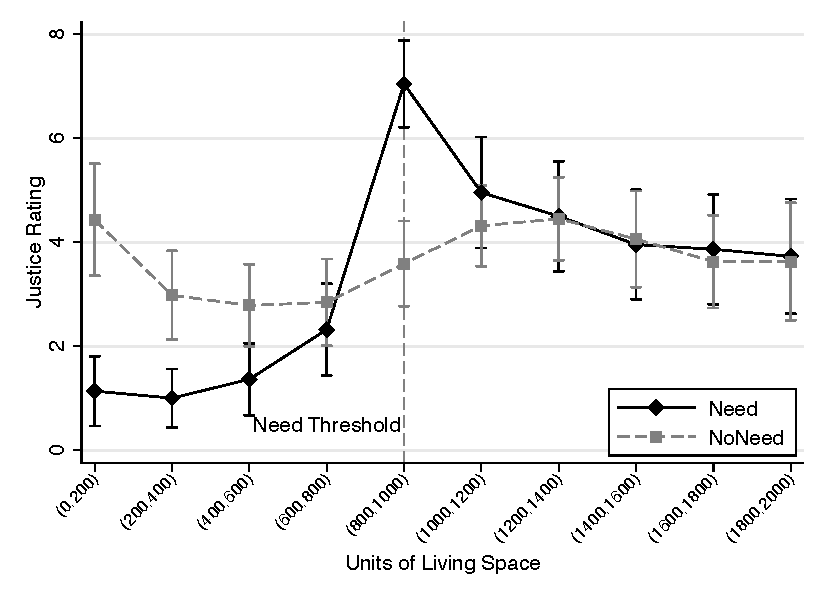
\includegraphics{figures/figure_13.pdf}
   \begin{minipage}{\linewidth}
      \footnotesize
      \textit{The figure shows the mean justice ratings for $x=\{0,200,\ldots,2000\}$ units of living space on a $[0,1]$ scale and the respective $90\%$ confidence intervals of $n=44$ ($n=51$) participants in the global rating task of the Need (NoNeed) treatment. The solid (dashed) line represents the Weibull fit with $r=1000$ as reference point.}
   \end{minipage}
   \caption{Mean justice ratings in the global rating task (conditional sample)}
   \label{fig:figure_13}
\end{figure}

\clearpage
\begin{table}[ht!]
   \centering
   \caption{Mean justice ratings in the global rating task by treatment (conditional sample}\label{tab:global_ratings_conditional}
   \begin{tabular}{rd{1.3}d{1.3}cd{1.3}d{1.3}cd{2.3}d{1.3}d{1.3}}                                                                                                                                                                     \\[-0.5ex]\hline
              & \multicolumn{2}{c}{Need}                              &   & \multicolumn{2}{c}{NoNeed}                            &   & \multicolumn{3}{c}{$t$ Test}                                                                  \\\cline{2-3}\cline{5-6}\cline{8-10}
      Units   & \multicolumn{1}{c}{Mean}   & \multicolumn{1}{c}{SE}   &   & \multicolumn{1}{c}{Mean}   & \multicolumn{1}{c}{SE}   &   & \multicolumn{1}{c}{Mean Diff.}   & \multicolumn{1}{c}{SE}   & \multicolumn{1}{c}{$p$}         \\\hline\hline
         0    & 0.013                      & 0.011                    &   & 0.046                      & 0.027                    &   & -0.033                           & 0.031                    & 0.291                           \\
       200    & 0.048                      & 0.014                    &   & 0.151                      & 0.032                    &   & -0.103                           & 0.037                    & 0.007                           \\
       400    & 0.081                      & 0.020                    &   & 0.219                      & 0.033                    &   & -0.138                           & 0.040                    & 0.001                           \\
       600    & 0.140                      & 0.027                    &   & 0.324                      & 0.038                    &   & -0.184                           & 0.048                    & 0.000                           \\
       800    & 0.224                      & 0.037                    &   & 0.395                      & 0.040                    &   & -0.171                           & 0.053                    & 0.002                           \\\hline
      1000    & 0.664                      & 0.043                    &   & 0.496                      & 0.037                    &   &  0.169                           & 0.057                    & 0.004                           \\
      1200    & 0.742                      & 0.039                    &   & 0.616                      & 0.026                    &   &  0.126                           & 0.052                    & 0.017                           \\
      1400    & 0.832                      & 0.026                    &   & 0.695                      & 0.033                    &   &  0.136                           & 0.043                    & 0.002                           \\
      1600    & 0.903                      & 0.018                    &   & 0.802                      & 0.028                    &   &  0.101                           & 0.034                    & 0.004                           \\
      1800    & 0.949                      & 0.009                    &   & 0.882                      & 0.025                    &   &  0.067                           & 0.028                    & 0.020                           \\
      2000    & 0.980                      & 0.008                    &   & 0.972                      & 0.011                    &   &  0.008                           & 0.014                    & 0.567                           \\\hline
      \multicolumn{10}{p{13cm}}{\footnotesize\textit{The table shows the mean justice ratings of $x=\{0,200,\ldots,2000\}$ units of living space on a $[0,1]$ scale and the respective standard errors of $n=44$ ($n=51$) participants in the global rating task of the Need (NoNeed) treatment, and the results of a $t$ test (mean differences, standard errors, $p$ values) on the mean difference (Welch test). Positive (negative) mean differences indicate that the respective number of units of living space was rated as more (less) just in the Need treatment than in the NoNeed treatment.}}
   \end{tabular}
\end{table}

\clearpage
\begin{table}[ht!]
   \centering
   \caption{Fitted parameters of the Weibull distribution (conditional sample)}\label{tab:weibull_conditional}
   \begin{tabular}{ld{2.8}d{2.6}cd{2.6}d{2.6}}                                                                                                                  \\[-0.5ex]\hline
                              & \multicolumn{2}{c}{Need}                                     &   & \multicolumn{2}{c}{NoNeed}                                   \\\cline{2-3}\cline{5-6}
      Parameter               & \multicolumn{1}{c}{$r=0$}   & \multicolumn{1}{c}{$r=1000$}   &   & \multicolumn{1}{c}{$r=0$}   & \multicolumn{1}{c}{$r=1000$}   \\\hline\hline
      $\lambda_0$             &   0.00091^{***}             &   0.00047^{***}                &   &   0.00085^{***}             &   0.00056^{***}                \\
                              &  (0.00001)                  &  (0.00015)                     &   &  (0.00002)                  &  (0.00013)                     \\[1ex]
      $\lambda_1\times D$     &                             &   0.00056^{***}                &   &                             &   0.00025^{*}                  \\
                              &                             &  (0.00015)                     &   &                             &  (0.00013)                     \\[1ex]
      $k_0$                   &   2.84639^{***}             &   1.44034^{***}                &   &   1.50106^{***}             &   0.87042^{***}                \\
                              &  (0.15670)                  &  (0.37578)                     &   &  (0.08633)                  &  (0.17041)                     \\[1ex]
      H0: $p(k_0\le 1)$       &   0.000                     &   0.242                        &   &   0.000                     &   0.447                        \\[1ex]
      $k_1\times D$           &                             &   0.25428                      &   &                             &   1.15519^{***}                \\
                              &                             &  (0.42271)                     &   &                             &  (0.25941)                     \\[1ex]
      H0: $p(k_0+k_1\le 1)$   &                             &   0.000                        &   &                             &   0.000                        \\\hline
      $n$                     & 484                         & 484                            &   & 561                         & 561                            \\
      $\bar{R}^2$             &   0.9252                    &   0.9322                       &   &   0.8692                    &   0.8729                       \\
      $RMSE$                  &   0.1799                    &   0.1712                       &   &   0.2276                    &   0.2243                       \\\hline
      \multicolumn{6}{p{13cm}}{\footnotesize\textit{The table shows the results of fitting a Weibull distribution to the participants' justice ratings in the global rating task using nonlinear OLS by treatment. $D=0(1)$ for $x<(\ge )1000$ units of living space. First row: means, second row: standard errors. Significance levels: $^{*}p\le 0.10$, $^{**}p\le 0.05$, $^{***}p\le 0.01$.}}
   \end{tabular}
\end{table}


%%%%%%%%%%%%%%%%%%%%%%%%%%%%%%%%%%%%%%%
% MEAN RATINGS RELATIVE (CONDITIONAL) %
%%%%%%%%%%%%%%%%%%%%%%%%%%%%%%%%%%%%%%%
\clearpage
\section{Mean Justice Ratings in the Relative Rating Task: Conditional Sample}\label{sec:app_conditional_relative}
\begin{figure}[ht!]
   \centering
   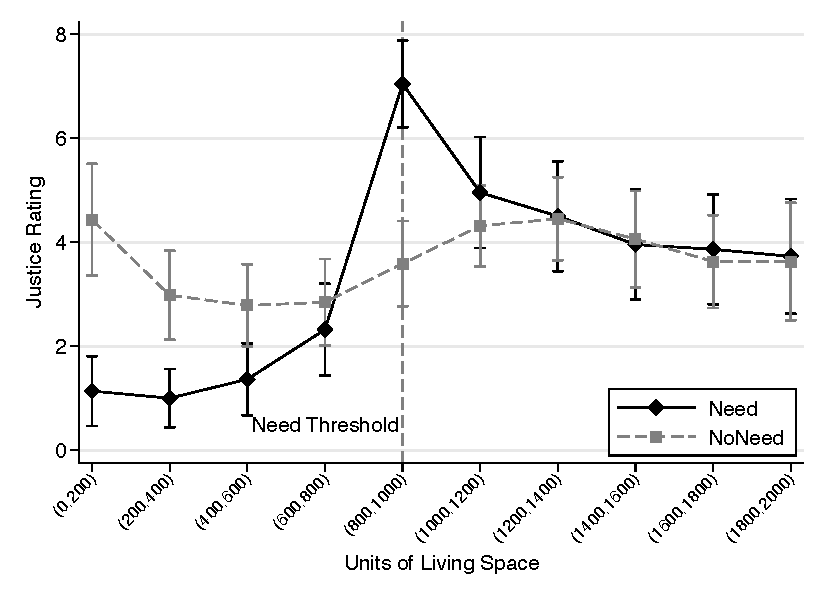
\includegraphics{figures/figure_14.pdf}
   \begin{minipage}{\linewidth}
      \footnotesize
      \textit{The figure shows the mean justice ratings of comparing two adjacent endowments with $\{(0,200),(200,400),\ldots,(1800,2000)\}$ units of living space on a $[-11,+11]$ Likert scale and the respective $90\%$ confidence intervals of $n=44$ ($n=51$) participants in the relative rating task of the Need (NoNeed) treatment. Positive (negative) numbers indicate that the larger endowment was rated as more (less) just than the smaller endowment.}
   \end{minipage}
   \caption{Mean justice ratings in the relative rating task (conditional sample)}
   \label{fig:figure_14}
\end{figure}

\clearpage
\begin{table}[ht!]
   \centering
   \caption{Mean justice ratings in the relative rating task by treatment (conditional sample)}\label{tab:relative_ratings_conditional}
   \begin{tabular}{ld{1.2}d{1.2}cd{1.2}d{1.2}cd{2.2}d{1.2}d{1.3}}                                                                                                                                                                      \\[-0.5ex]\hline
                    & \multicolumn{2}{c}{Need}                              &   & \multicolumn{2}{c}{NoNeed}                            &   & \multicolumn{3}{c}{$t$ Test}                                                             \\\cline{2-3}\cline{5-6}\cline{8-10}
      Units         & \multicolumn{1}{c}{Mean}   & \multicolumn{1}{c}{SE}   &   & \multicolumn{1}{c}{Mean}   & \multicolumn{1}{c}{SE}   &   & \multicolumn{1}{c}{Mean Diff.}   & \multicolumn{1}{c}{SE}   & \multicolumn{1}{c}{$p$}         \\\hline\hline
         (0,200)    & 1.14                       & 0.40                     &   & 4.43                       & 0.64                     &   & -3.30                            & 0.78                     & 0.000                           \\
       (200,400)    & 1.00                       & 0.33                     &   & 2.98                       & 0.51                     &   & -1.98                            & 0.63                     & 0.002                           \\
       (400,600)    & 1.36                       & 0.41                     &   & 2.78                       & 0.47                     &   & -1.42                            & 0.64                     & 0.028                           \\
       (600,800)    & 2.32                       & 0.53                     &   & 2.84                       & 0.50                     &   & -0.52                            & 0.70                     & 0.470                           \\
       (800,1000)   & 7.05                       & 0.50                     &   & 3.59                       & 0.49                     &   &  3.46                            & 0.70                     & 0.000                           \\\hline
      (1000,1200)   & 4.95                       & 0.63                     &   & 4.31                       & 0.46                     &   &  0.64                            & 0.77                     & 0.409                           \\
      (1200,1400)   & 4.50                       & 0.63                     &   & 4.45                       & 0.47                     &   &  0.05                            & 0.78                     & 0.950                           \\
      (1400,1600)   & 3.95                       & 0.63                     &   & 4.06                       & 0.55                     &   & -0.10                            & 0.83                     & 0.900                           \\
      (1600,1800)   & 3.86                       & 0.63                     &   & 3.63                       & 0.53                     &   &  0.24                            & 0.82                     & 0.774                           \\
      (1800,2000)   & 3.73                       & 0.66                     &   & 3.63                       & 0.67                     &   &  0.10                            & 0.95                     & 0.916                           \\\hline
      \multicolumn{10}{p{13cm}}{\footnotesize\textit{The table shows the mean justice ratings comparing two adjacent endowments with $\{(0,200),(200,400),\ldots,(1800,2000)\}$ units of living space on a $[-11,+11]$ Likert scale of $n=44$ ($n=51$) participants in the relative rating task of the Need (NoNeed) treatment, and the results of a $t$ test (mean differences, standard errors, $p$ values) on the mean difference (Welch test). Positive (negative) means indicate that the larger endowment was rated as more (less) just than the smaller endowment. Positive (negative) mean differences indicate that the respective comparison was rated as more (less) just in the Need treatment than in the NoNeed treatment.}}
   \end{tabular}
\end{table}


%%%%%%%%%
% TEXTS %
%%%%%%%%%
\clearpage
\section{Vignette Texts}\label{sec:app_vignette}


%%%%%%%%%%%%%%%%
% INTRODUCTION %
%%%%%%%%%%%%%%%%
\subsection*{Introduction Screen}
\noindent Welcome to our study,

In this study on justice, we are interested in your opinions and assessments.
Therefore, we will present to you a number of varying scenarios, and we ask you to imagine them as real.
Please take the time to place yourself into the scenarios and to come to your own personal assessment.
In this study, there are no right or wrong answers.

We will assess your evaluations as well as the evaluations of all other participants in this study.
All data will be saved anonymously so that no details can be attributed to any person.
The results of the study will be published.
Thereby they will influence future research and shall be used to inform politics.


%%%%%%%%%%%%
% VIGNETTE %
%%%%%%%%%%%%
\subsection*{Vignette Texts of the Need and NoNeed Treatments}
\textit{Note: The vignette texts of the Need and NoNeed treatments differ only on the information given with regards to needs, which was left out in the NoNeed treatment, as is indicated in the following by square brackets.}

\medskip{}
\noindent Please imagine the following:

In the region of Bergtal, a new village is going to be established.
It is the task of the Public Housing Association of Bergtal to build housing.

All households in this region want to live in the largest living space possible.
{[}The residents of the region have collectively decided on a minimum amount of living space, under which living a decent life in this community is not possible.{]}
Between the households in the region, there are no noteworthy differences {[}and the minimum amounts are the same for each household: Each household should have $1000$ regional---i.\,e., common to the region---area units of living space in order to be able to live a decent life.
To have a living space with the equivalent area means for a household to live in close quarters, but it will be just enough to lead a decent life{]}.

There are enough means to be able to build up to $2000$ regional area units of living space for each household.
The Regional Parliament decides how much living space will actually be built for the residents of the new village.
The decision has otherwise no noteworthy consequences.
For the construction of living space, no additional area would be consumed.
The new village will be built in the area of an old village that was abandoned after a fire destroyed the houses.

In its decision, the Regional Parliament wants to take into account how impartial people---like you---judge the justice of different scenarios.
Your task is, therefore, to indicate for each scenario how just you hold the distribution of living space to be.


%%%%%%%%%
% TASKS %
%%%%%%%%%
\subsection*{Task Descriptions of the Need and NoNeed Treatments}
\textit{Note: Participants received two different task descriptions, one for the justice evaluations of the 11 scenarios each for themselves (global rating task) and one for the pairwise evaluations (relative rating task).}

\subsubsection*{Global Rating Task}
The following scenarios differ in how much living space shall be built for each household according to the decision of the Regional Parliament.

Please indicate for each following distribution how just you regard it to be.
$100$ percent means that you judge the distribution to be completely just.
Percentages close to $100$ percent mean that you judge the distribution to be almost completely just.
Percentages far from $100$ percent mean that you judge the distribution to be significantly less just.
Please familiarize yourself now with each of the given distributions before answering the questions.

\subsubsection*{Relative Rating Task}
On the coming pages, we will present to you each time two differing scenarios.
We will ask you furthermore to indicate on a scale from 1 (equally just or unjust) to 11 (much more just) how just you regard each scenario compared to the other one to be.


\end{document}

\begin{landscape}
   \begin{table}[ht!]
      \centering
      \caption{Individual classification of participants}\label{tab:classification}
      {\normalsize\small
         \begin{tabular}{lclccl}\hline\\[-1.5ex]
            Type             & \multicolumn{2}{c}{Need}                     &   & \multicolumn{2}{c}{NoNeed}                      \\\cline{2-3}\cline{5-6}
                             & Number   & Subject IDs                       &   & Number   & Subject IDs                          \\\hline\hline
            Hump-Shaped      &  8       & 2, 14, 15, 19, 26, 36, 37, 42     &   &  2       & 10, 28                               \\[2ex]
            Binary           &  4       & 20, 27, 28, 41                    &   &  5       & 6, 13, 23, 37, 42                    \\[2ex]
            Flat at/above    &  7       & 1, 17, 32, 40, 44, 47, 51         &   &  1       & 12                                   \\
            Need Threshold   &          &                                   &   &          &                                      \\[2ex]
            Zero below       & 15       & 3, 5, 10, 11, 12, 13, 23, 25,     &   &  5       & 3, 11, 19, 20, 50                    \\
            Need Threshold   &          & 29, 30, 31, 35, 45, 48, 50        &   &          &                                      \\[2ex]
            Increasing       & 17       & 4, 6, 7, 8, 9, 16, 18, 21,        &   & 36       & 1, 2, 6, 7, 8, 9, 14, 15             \\
                             &          & 22, 24, 34, 38, 39, 43, 46, 49,   &   &          & 16, 17, 21, 24, 25, 27, 29, 30,      \\
                             &          & 52                                &   &          & 31, 32, 33, 35, 36, 38, 39, 40,      \\
                             &          &                                   &   &          & 41, 43, 45, 46, 47, 48, 49, 52,      \\
                             &          &                                   &   &          & 53, 54, 55, 56                       \\[2ex]
            Other            &  1       & 33                                &   &  8       & 4, 22 (Egalitarian)                  \\
                             &          &                                   &   &          & 51 (Neg. Egalitarian)                \\
                             &          &                                   &   &          & 18, 22, 26, 34, 44, 57 (Irregular)   \\\hline
      \end{tabular}}
   \end{table}
\end{landscape}
